\documentclass[../dejiny-rodu-prusiku.tex]{subfiles}

\begin{document}

% str 209 @ 242
\chapter{Větev Stražiště}

Zakladatel: Vojtěch Prusík 1790 - 1867

Vysoko nad říčkou Střelou s mnoha stran obklopena lesy, leží vesnička Stražiště. Již v šerém dávnověku bylo zde sídliště a hranice přemyslovského státu českého. Při nebezpečí nepřátelského vpádu se zde zapalovaly ohně a od těch časů říká se zde Stražiště. Takových míst je v Čechách hojně. Stražiště ve XII. století patřilo vladykům z Potvorova. Dlouho pak bylo majetkem kláštera v Plasích a také pana Hrobčíckého ze Všesulova. Od roku. 1672 stal se majitelem hrabě Karel Maxmilián Lažanský z Manětína, který koupil Stražiště a řadu jiných vesnic od Václava Karla z Hoslan. Tato vesnička byla vždy malá, po třicetileté válce žili zde jen čtyři osad­níci, dnes jich tam je také ke stu. Farní kostel svatého Martina, s jehož dvou věží je výhled do dalekého, půvabného kraje na lesy a romantická údolí Střely, připomíná se již v roce 1250. Do této vesnice přistěhoval se kolem roku 1788, tedy za císaře Josefa II., člen našeho rodu Adam Prusík. Zmínili jsme se již o něm na strán­ce 12 v kapitolce o Plasích a jejich významu pro rod Prusíků.

Adam Prusík byl vnukem Václava Prusíka narozeného v Sedlci. Adam byl vyučený zedník a měl čtyři syny. Dcerky zemřely v dětství. Zednickému řemeslu naučil se u své­ho otce Evžena Prusíka, který byl stavitelem a malířem kláštera v Plasích v době jeho největší slávy v XVIII. století. Evžen Prusík, otec Adamův nepracoval jen v Plasích, ale zúčastnil se i stavby a přestavby mnoha kostelů. Kdo z členů rodu zavítá do Kožlan, uzří tam kostel sv. Vavřince. Kdo jede z Plas do Kralovic, uvidí již od sochy sv. Jana uprostřed mírně zvlněného kraje památnou Mariánskou Týnici, která jako drahokam byla zasazena v pruhovaných polích smaragdových, vroubených pásem modrých lesů hubenovských. Na překrásné stavbě českého baroka Mariánské Týníce v XVIII. století, jednom z nejslavnějších poutních míst v Čechách, podílel se zrovna jako v Kožlanech Evžen Prusík z Plas.

I Adam Prusík, syn Evženův, byl velmi činný ve stavebnictví, ale více již pracoval na stavbách civilních, zvláště také proto, že zrušením kláštera v Plasích, když mu bylo 20 let, ustával také obrovský stavební a umělecký vývoj církevní. Nejstarším synem Adamovým, usazeným ve Stražišti, byl Vojtěch. Narodil se 22. 4. 1790 a u otce vyučil se zednickému řemeslu. Jeden čas míval ve Stražišti i malý hostinec. Již jeho matka byla Němkou a on si vzal za manželku rovněž Němku Annu Sieberovou nar. v roce 1794 v Kalci.  Její otec tam byl šafářem. Důsledkem tohoto českoněmeckého manželství bylo, že mnozí potomci se poněmčili nebo si vzali opět Němky a odnárodnění se tak zpečetilo. Vojtěch Prusík ve Stražišti měl šest dětí.

% str 210 @ 243
Byli to synové František, Antonín, Josef, Václav a Jan a dcera Anna. Ostatní jejich děti, které nedožily alespoň deseti let života, nejmenujeme. Vojtěch Prusík zemřel na marasmus 24. 7. 1867 ve Stražišti. Stal se zakladatelem větve "Stražiště" jako zase jeho bratr Josef je zakladatelem větve "Jihlava" a bratr Jan zakladatelem větve "Kuchyně u Herálce". Je zajímavé, že o členech těchto větví i když byly ve své době dosti početné, členům ostatních nejsilnějších rodových větví nenapadlo ani, že by všichni by­li mezi sebou spřízněni. Důvod k těmto pochybnostem, byl asi vždy ten, že mnozí Prusíci patřící k větvím Stražiště, Jihlava nebo Kuchyně stali se Němci, žili v cizině a nevěřilo se dlouho, že by patřili k rodu jehož základní kmen byl čistě slovanský a pocházel z české vesnice Sedlec u Plas.

Manželka Vojtěcha Prusíka zemřela ve Stražišti 26. 12. 1876 a v té době žil s ní pouze syn Antonín.

Nejstarším synem Vojtěcha Prusíka, zednického mistra ze Stražiště byl František. Narodil se 8. 8. 1824. Vyučil se pekařem. Za manželku měl opět Němku, která ač žila s mužem většinou v českých obcích se pořadně česky nikdy nenaučila. Byla to Josefa Neumannová narozena v Toužimi 21. 1. 1823. Pekař František Prusík oženil se 22. 10. l850 a pracoval a žil pokud je známo, v těchto místech: Borek u Žlutic, Rabštejn, Nový dvůr u Rabštejna, Trnová, Plasy a Stražiště. František Prusík se svou ženou Josefou měli sedm dětí. Byly to tři dcery a čtyři synové. František Prusík onemocněl v roce 1887 zánětem slepého střeva a v několika dnech zemřel ve svém rodišti Stražišti. Až do posledních chvil pracoval. Vdova po něm žila pak u syna v Teplicích a tam zemřela za první světové války 11. 2. 1915.

Nejstarším dítětem Františka Prusíka byla dcera Barbora. Narodila se 4. 3. 1850 v Borku u Žlutic. Poněvadž asi lépe mluvila německy než česky, odebrala se za lepším živobytím do Vídně, kam tolik lidí z Čech a Moravy v XIX. století se stěhovalo. Vždyť to bylo lákavé sídlo mocnářství rakousko-uherského, příležitost k výdělkům byla jistě veliká a tak mnohý neodolal pokušení, aby tam neodešel. Barbora Prusíková se dvakrát provdala. Po prvé Bailová. Z tohoto manželství narodila se dcera Marie 7. 8. 1878 ve Vídni. Zůstala svobodná a zemřela v listopadu 1958 v Domově starých lidí ve Vídni XIII. Lainz. Druhou dcerou byla Julie nar. 24. 1. 1886. Je provdaná Schwögerová, bydlí ve Vídni II, Leopoldgasse 6. Má syna Josefa nar.1914. Z druhého manželství, kdy byla provdaná za dělníka Bělohlávka, narodila se dcera Aloisie 14. 10. 1892. Byla Provdaná Braunseisová. Bydlí ve Vídni XII, Böckhgasse 4. Má jednu dceru Luisu nar. 2. 3. 1922 provdanou Křenovou. Ta má dvě dcery, Gabrielu nar. 25. 4. 1947, která je provdaná Bednářová ve Vídni XVl, Brüsselgasse 43. Má dceru Andreu, nar. v červenci 1965. Druhou dcerou Luisy Krenové
% str 211 @ 245
nové je dcera Eva nar. 21. 11. 1954. Luisa je nyní v ošetřovaní psychiatrické léčebny ve Vídni. Barbora Bělohlávková zemřela ve Vídni 18. 11. 1929. Dalším dítětem pekaře Františka Prusíka, byl syn František. Narodil se v Rabštejně v roce 1851. Vyučil se truhlářství a žil od mladých let ve Vídni. Za manželku měl Češku Marii Královou nar. 8. 9. 1854 v Martinicích u Dolních Kralovic. František Prusík v pozdějších svých letech nevedl však pořádný život, značně propadl alkoholu a žena odešla do Čech, kde zemřela v Praze na Žižkově 31. 1. 1929. Vlastních dětí neměli. Truhlář František Prusík zemřel opuštěn svými příbuznými ve Vídni v Domové starých lidí 13. 3. 1922.

% str 210+1 @ 244
\begin{figure}
\centering
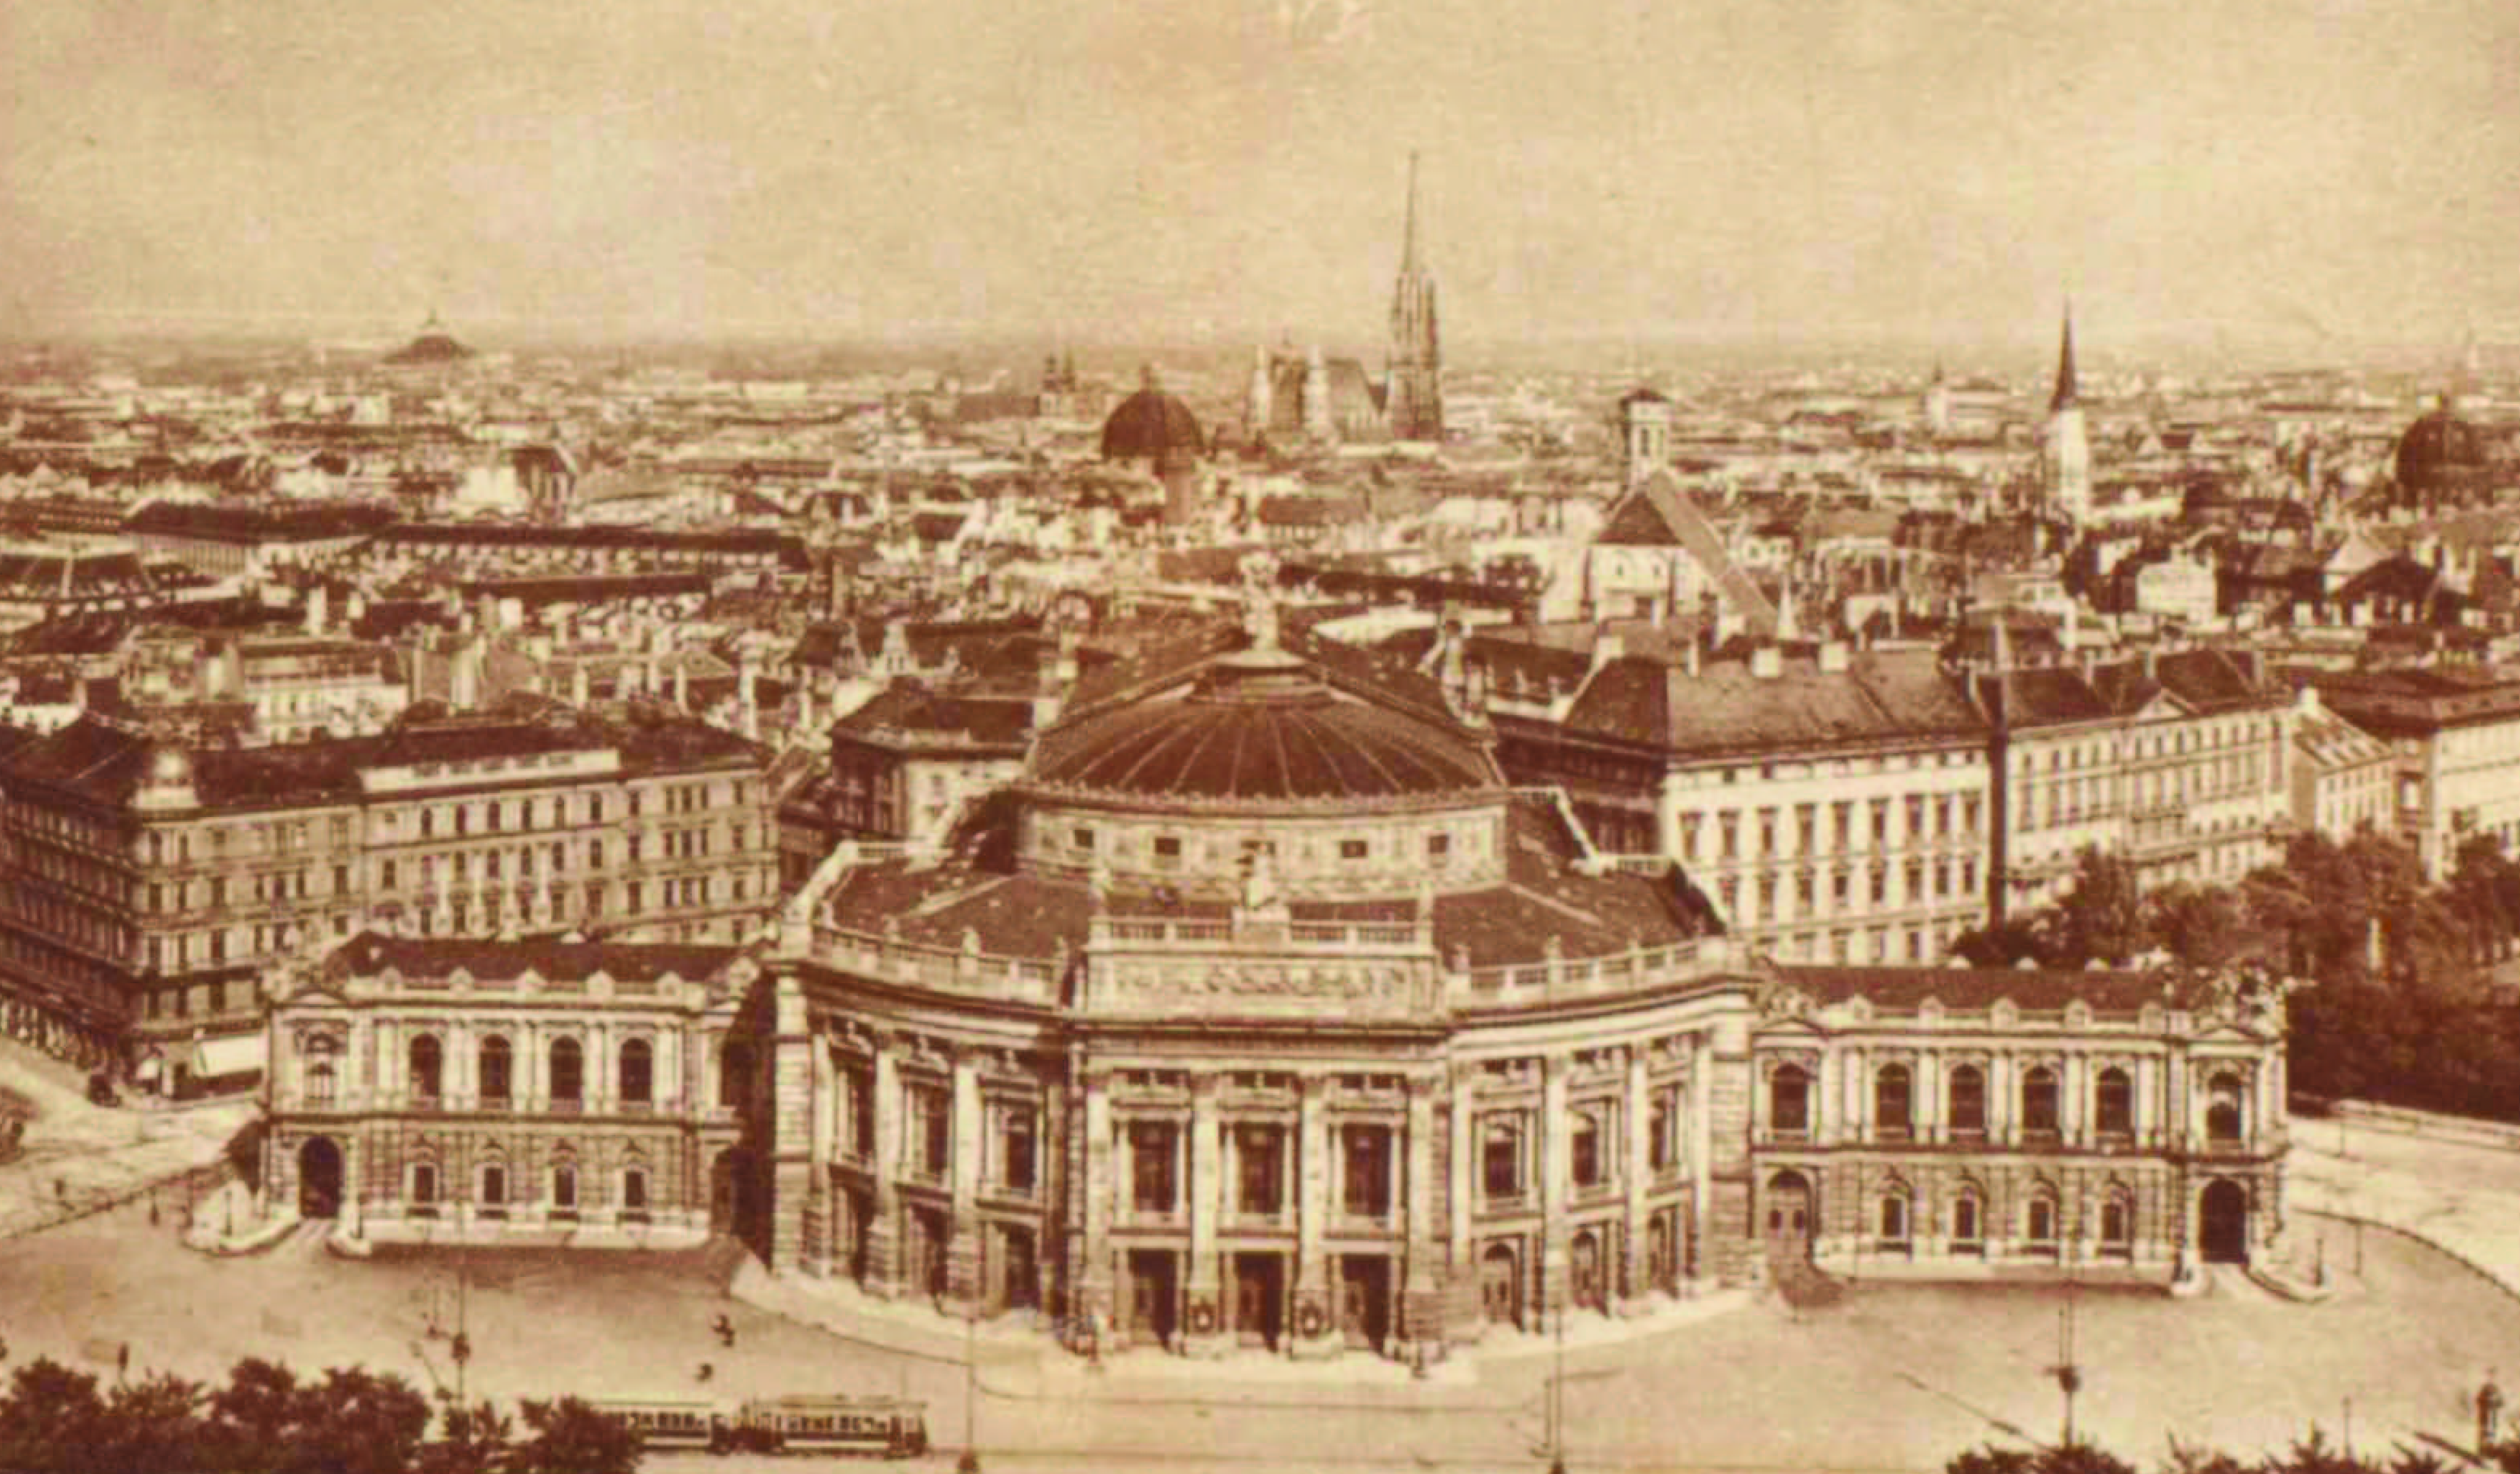
\includegraphics[width=\textwidth, height=\textheight, keepaspectratio]{244-a-pohled_na_viden}
\caption{Pohled na Vídeň, kde žili a žijí členové rodu}
\label{fig:244-a-pohled_na_viden}
\end{figure}

             \begin{figure}
\centering
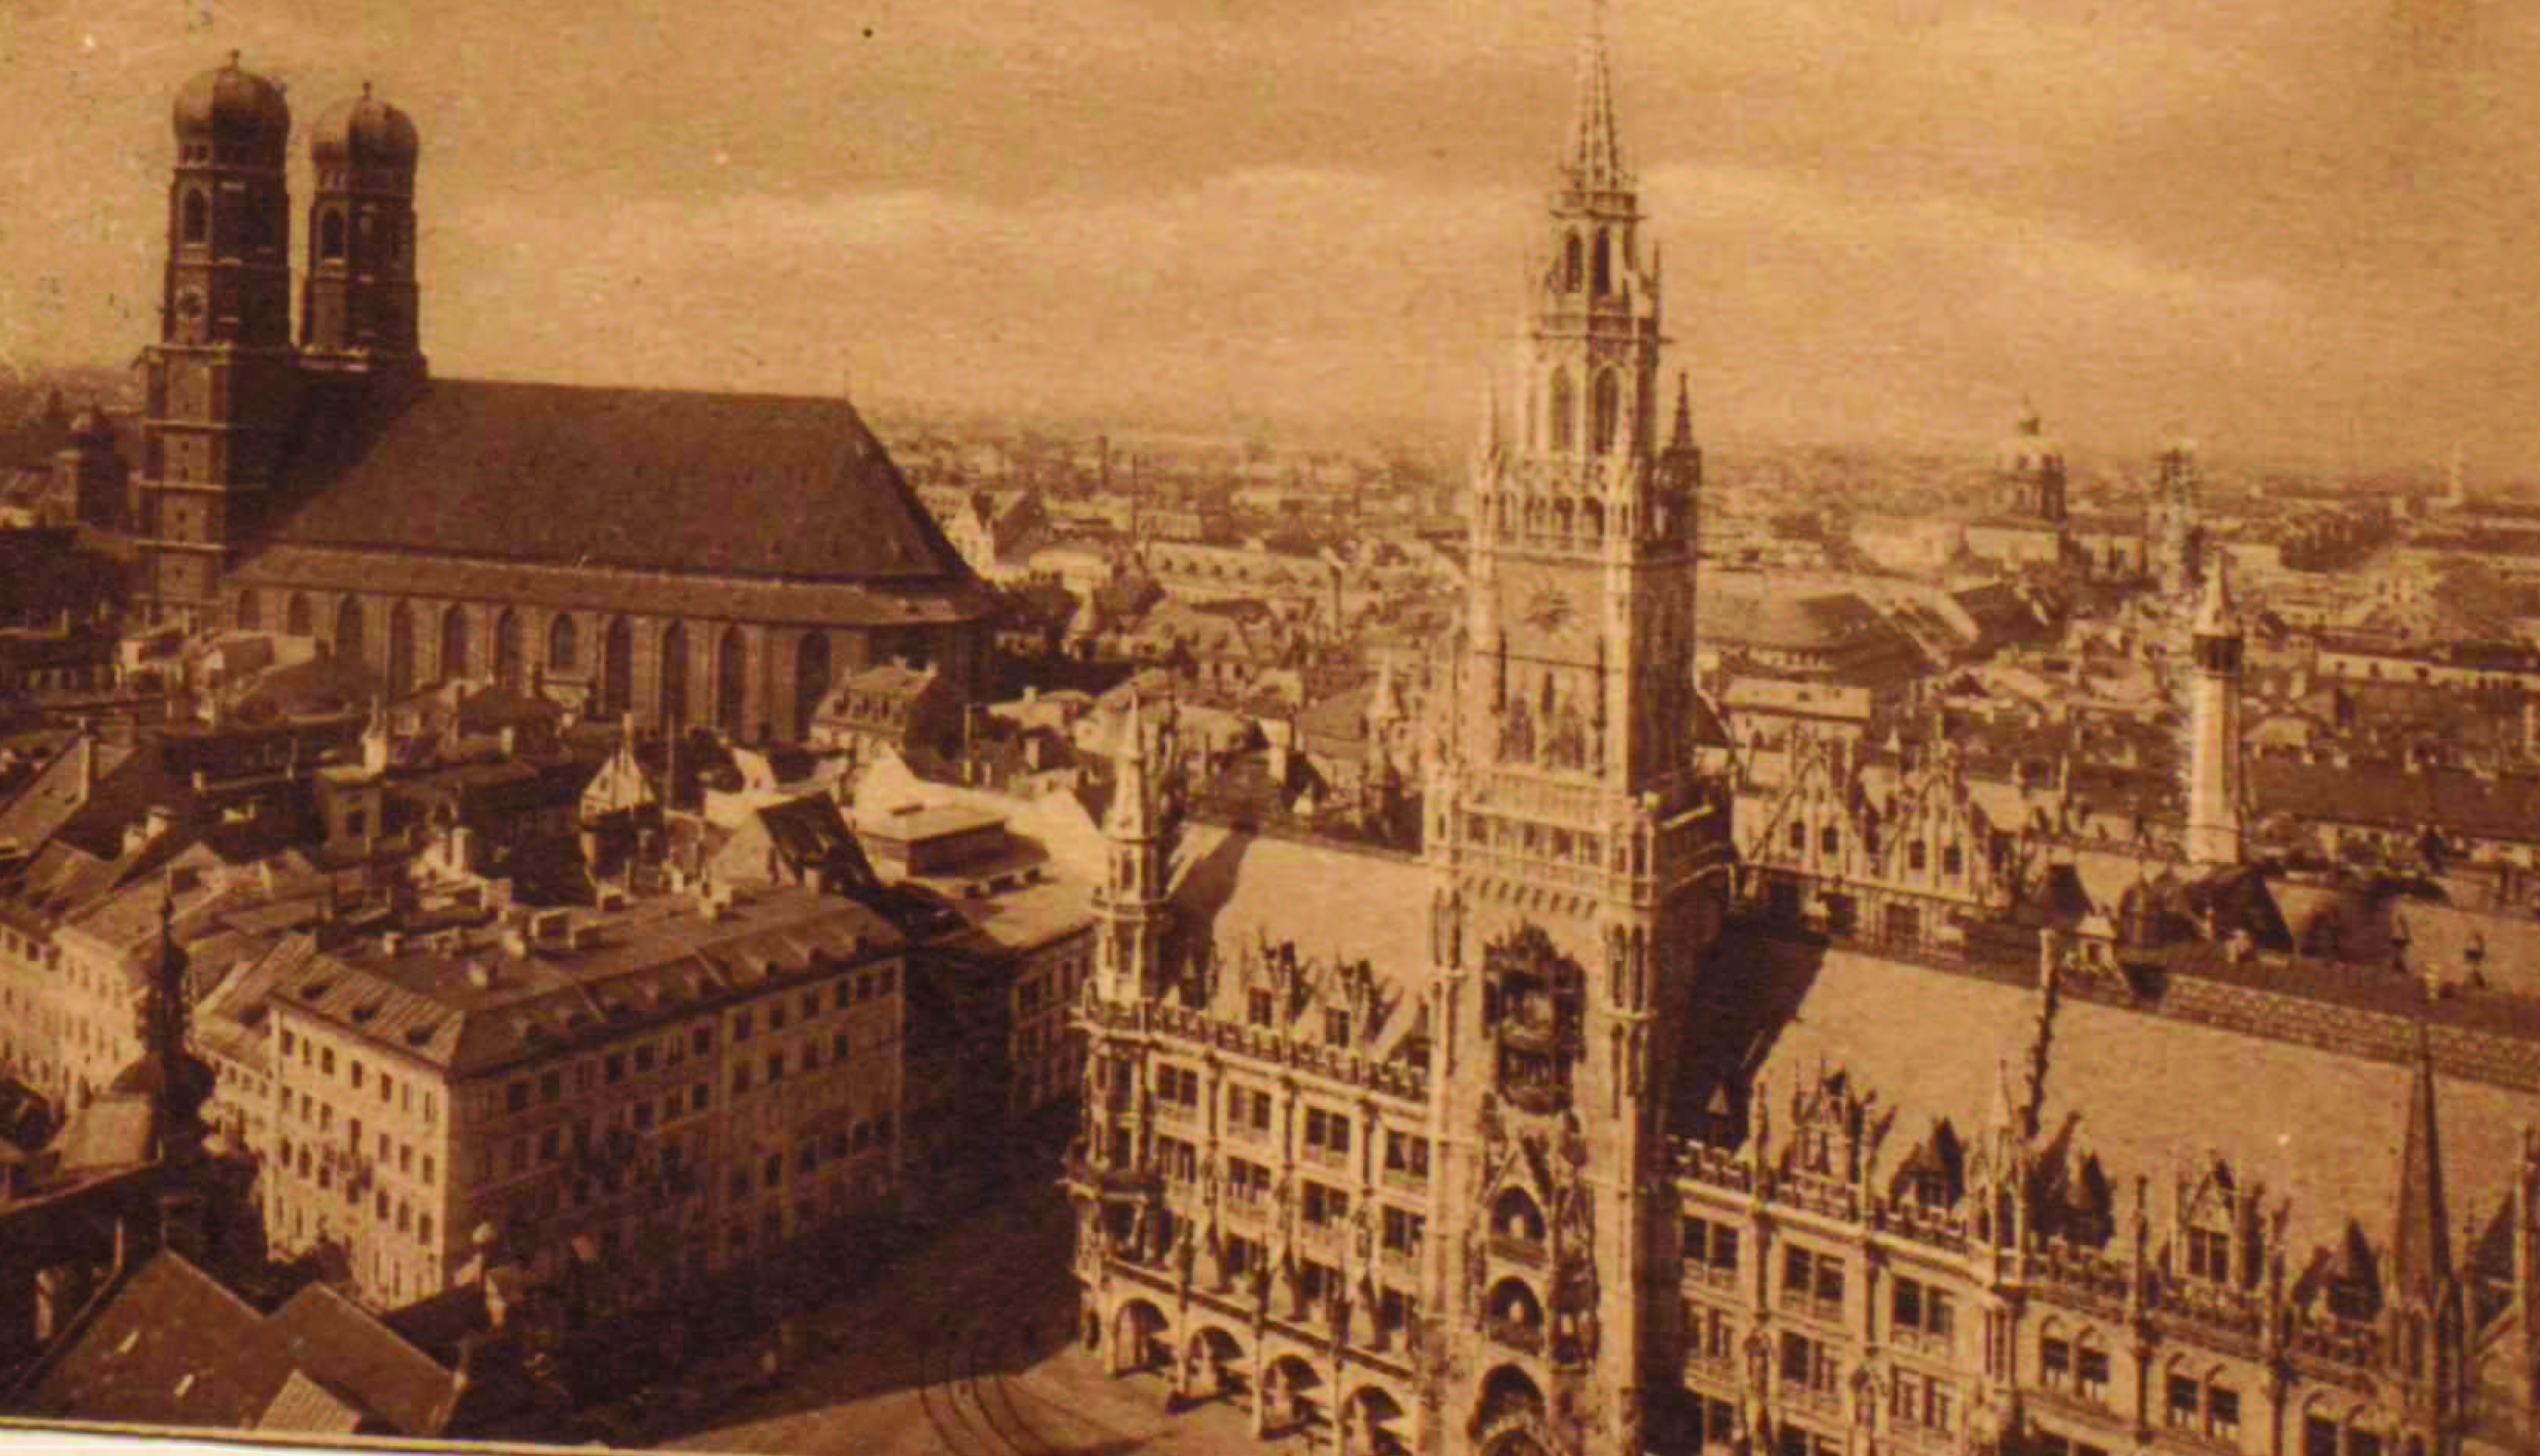
\includegraphics[width=\textwidth, height=\textheight, keepaspectratio]{244-b-mnichov}
\caption{Mnichov, kde žijí členové rodu Ing. Gerhard Prusik a Jan Prokop}
\label{fig:244-b-mnichov}
\end{figure}

% str 211 @ 245 (pokr.)
Dalším synem Františka Prusíka byl Antonín. Narodil se 7. 10. 1853 v Novém dvoře u Žíhle, nedaleko Rabštejna. To je vlastně jediný, který ze všech potomků. Františka Prusíka, nar. v roce 1824 ve Stražišti, zůstal zcela věren českému národu. Antonín Prusík vyučil se tesaři­ně, ale poměrně brzy byl přijat do služeb drah. Působil v Plasích, dlouho také v železničním strážním domku mezi Mladoticemi a Přehořovem na katastru obce Řemešín. Ke konci života žil u svého syna v Mladoticích ve vlastním domku. Manželkou jeho byla Tekla Šmídová nar. 23. 9. 1852 v Plasích. Zemřela již za první světové války 23. 12. 1916. Antonín s Teklou měli pět synů. Po smrti své manželky se již neoženil a byl přes čtvrt sto­letí vdovcem. Život ho nakonec omrzel a 7. 10. 1942 v den svých narozenin skočil pod vlak v Mladoticích. Antonín Prusík byl veselý člověk, velmi oblíbený, od dětství dovedl německy a se svými sourozenci se rád stýkal, přestože národnostně se rozdělili.

Nejstarším synem Antonína Prusíka byl Heřman. Narodil se 7. 4. 1879 v Plasích. Téměř celý život byl zaměstnán u dráhy. Nejdříve byl v Plasích, pak v Kokšíně u Švihova. Za první světové války byl dva roky v Polsku u železnič­ního pluku. Po válce sloužil pak u dráhy ve strážním domku u obce Přehořova a odtud odešel do pense do Plzně v roce 1933, kde si koupil rodinný domek na Božkově. Manželkou jeho byla Anna Mikutová nar. 7. 9. 1878 v Chrašťovicích. Zemřela 21. 3. 1949 a Heřman Prusík pak za šest let po ní dne 25. 6. 1955. Je pozoruhodné, že strážní domek, kde Heřman Prusík působil, byl za statkem kde hospodařil Václav Prusík v Přehořově. Byli spolu dobří přáte­lé, často se podivovali že mají stejné příjmení, ale nikdy nevěděli, že jsou vzájemně spříznění, i když vzdáleně. Heřman Prusík měl jediného syna. Byl to Antonín Prusík, nar. 31. 7. 1904 v Plasích. Byl vyučen tak zvanému černému ře­meslu, dlouho byl také garážmistrem u KNV v Plzni. Dnes žije na odpočinku v domku svých rodičů v Plzni-Božkově, Jiráskova 27. Manželkou jeho je Marie Bezděková narozená v Olešnici v Sasku 10. 11. 1907. Brzy ovšem po jejím narození vrátili se její rodiče do Čech. Antonín Prusík má dvě děti. Dcera Věra nar. 12. 8. 1930 v Plzni je provdaná
% str 212 @ 246
Šlaisová, nyní je rozvedená. Je úřednicí v plzeňském pivovaru měšťanském. Má dcerku Ivanu nar. 4. 12. 1957. Druhé dítě Antonína Prusíka je syn Zdeněk. Narodil se 3. 7. 1935 v Plzni, je konstruktérem ve Škodovce. Bydlí v Plzni-Doubravce, K špitálskému lesu 14. Jeho man­želkou  je Růžena Vorlová nar. 2. 12. 1941 ve Šťáhlavech u Plzně. Mají dcerku Janu Prusíkovou nar. 28. 11. 1963.

Druhým synem Antonína Prusíka, který se narodil v No­vém dvoře u Žíhle, byl Vincenc. Narodil se 3. 7. 1881 v Plasích. Vyučil se obuvníkem a pracoval také na různých místech ve Vídni. Z první světové války se vrá­til jako ruský legionář, přiženil se do Chrašťovic, kde jeho nastávající žena Ludmila Churavá, nar. 26. 2. 1890 (zemřela 21. 7. 1968) měla čtyřhektarové hospodářství. V zimě Vincenc Prusík provozoval svoje řemeslo. Později byl zaměstnancem silniční správy jako cestář, ale za okupace nesměl toto místo jako bývaly legionář zastávati a tak jen hospodařil. Vincenc Prusík měl syna Václava, dcerka Božena zemřela v dětství. V Chrašťovicích byl Vincenc Prusík velmi oblíben a o svých předcích po otci měl poměrně nejlepší přehled ze svých sourozenců. Zemřel náhle 15. 8. 1959. Byl pohřben ve Stražišti. Jeho syn Václav nar. 15. 9. 1922 bydlil s matkou v Chrašťovicích č. 12. Zůstal svobodný a je zaměstnancem dráhy v Mladoticích.

Třetí syn Antonínův jmenoval se Rudolf Prusík. Narodil se 24. 3. 1884 v Plasích. Také on dostal se ke dráze a nakonec působil v Mladoticích, kde měl domek a žil tam s rodiči. Jeho velkou zálibou byla myslivost. Za manžel­ku měl Marii Plevkovou nar. 24. 12. 1890. Pocházela z osa­dy Rouda u Žebnice. Zemřela v Mladoticích 26. 2. 1953 a její muž Rudolf Prusík odešel za ní na věčnost 5. 8. 1963. Rudolf Prusík měl se svou ženou Marií dvě děti. Syn Josef se narodil 29. 9. 1912. Vyučil se modelářem v Horní Bříze. Po květnu 1945 byl dosti angažován politicky, také zastupoval v samosprávě Mladotice a sousední vesnice. I on zdědil koníčka svého otce nimrodství. Za manželku měl Růženu Bulínovou nar. 1. 11. 1912 ve Výrově. Manželství se však nezdařilo a jeho manželka zemřela v roce 1958 ve Výrově. Josef Prusík, rodák z Mladotic, pracuje nyní ja­ko mistr v Keramických závodech v Horní Bříze a tam také bydlí v č. 408. Je bezdětný. Hlásí se s hrdostí k rodu. Sestrou Josefa Prusíka je Božena. Narodila se 13. 1. 1920 a za muže má Františka Buriána rodáka z Říčanska. Božena Buriánová roz. Prusíková je úřednicí ONV v Chebu, kde nyní bydlí v ulici Ztracená, číslo 12. Má dvě dce­ry. Její dcera Anna nar. 6. 10. 1940 je provdaná Stinglová a má synka Petra nar. 22. 11. 196l. Bydlí tam v Písečné ulici č. 12.

Druhá dcera je Věra narozená 14. 3. 1943 a bydlí také v Chebu, Mánesova 9. Je provdaná Blažková  a má dvě dě­ti. Její dcerka Ivana narodila se 10. 6. 1963 a syn Miroslav 13. 6. 1965.

% str 213 @ 247
Čtvrtým synem Antonína Prusíka byl Josef. Narodil se 3. 3. 1891 ve strážním domku železničním č. 33 u Řemešína. Byl zaměstnán v Žíhli, v Aši, Krýrech, Svojetíně a nakonec u dráhy v Kralovicích. Jeho man­želkou byla po prvé Marie Koldínská nar. v roce 1892 v Přívěticích u Radnic. Josef Prusík s ní však neměl děti. Zemřela v mladém věku 33 let v Plzni 26. 9. 1925. Josef Prusík se pak oženil znovu s Aloisií Birkovou 24. 11. 1907 v Kožlanech, kde její otec měl pilu. V Žíhli, kde byl Josef  Prusík také jeden čas staničním úředníkem, narodil se jim syn Jiří a na jiném působišti ve Svojetíně zase dcera Dagmar.

Za okupace úřadoval Josef Prusík na nádraží v Kralovicích, zúčastnil se odbojových akcí, byl na podzim 1944 zatčen a již 29. 12. 1944 zemřel v Terezíně. Jeho syn Jiří narodil se 10. dubna 1930 v Žíhlí. Je stavbyvedoucím u Pozemních staveb v Liberci, kde bydlí ve čtvrti V. Králův Háj č. 384. Jeho manželkou je Helena Neumannová nar. 29. 3. 1941 v Horce u Púchova na Sloven­sku. Je úřednicí. Zvláštní zálibou Jiřího Prusíka je sport, zejména sáňky a boby. Čilému sáňkařskému odboru v Liberci pomáhal také budovati závodní dráhu. Jiří Prusík je bezdětný.

Dcera Josefa Prusíka, který tak tragicky skončil, a jehož jméno je zaznamenáno na pamětních deskách na nádraží v Kralovicích a v Plzni, je Dagmar. Narodila se 5. 7. 1933 ve Svojetíně u Rakovníka. Svého otce si příliš nepamatuje. Pracuje ve zdravotnictví. Dnes je provdaná za lékaře Dufka ve Varnsdorfu, bydlí v čísle 1862. Dagmar Dufková roz. Prusíková je bezdětná a bydlí s ní matka.

Pátý syn Antonína Prusíka byl Jaroslav. Narodil se také přímo u kolejí ve strážním domku v Řemešíně 7. 6. 1894. I on byl zaměstnán u dráhy. Kromě Vincence Prusíka živila se tedy celá rodina Antonína Prusíka okřídleným kolem. Jaroslav Prusík měl však špatný osud. Jeho manželkou byla Aloisie Procházková nar. 28. 5. 1899 v Olešné u Rakovníka (zemřela 2. 2. 1969). Nejdéle působil Jaroslav v Novém dvoře u Stříbra, nynějších Pňovanech. Náhle Jaroslava zachvátila krční choroba a po operaci zemřel v mladém věku 9. 12. 1927. Měl jediného syna Ladislava, který se narodil 6. 5. 1925. Když otec zemřel, odstěhoval se s matkou do Žíhle a odtamtud zase v okupaci do Kaznějova. Je vyučen strojním zámečníkem a dnes pracuje u dráhy v Ústí nad Labem. Bydlí tam v pěkné vilce ve Střekově, Škrétova 3. Jeho manželkou je Vlasta Benešová nar. 8. 6. 1923 v Třemošné. Je úřednicí u dráhy. Jejich syn Ladislav nar. 25. 6. 1947, průmyslovák, je také nyní zaměstnán, aby tato tradice nevyšla z rodiny, u dráhy. Je svobodný.

Popsali jsme tedy krátce život potomků Antonína Prusíka, který jako jediný se z dětí Františka Prusíka, neodnárodnil.

% str 214 @ 248
Druhou dcerou Františka Prusíka, rodáka ze Stražiště, byla Matylda. Narodila se 14. 3. 1859 v Rabštejně. Také ona odstěhovala se brzy do Vídně, kde již byla její sestra Barbora. Provdala se tam za dělníka Josefa Zechnera a měla s ním dvě děti. Její dcera Františka Schaumayerová narodila se 9. 2. 1892. Žije ve Vídni XV. Flachgasse 11. Její syn František Schaumayer nar. 25. 6. 1917 je průvodčím elektrických drah ve Vídni. Je svobodný. Druhou dcerou Matyldy Zechnerové, roz. Prusíkové byla Amalie. Narodila se 29. 12. 1890 a provdala se za dělníka Brima. Zemřela však brzy 10. 2. 1927. Měla syna Františka nar. 1910 ve Vídni. František Brim děti nemá. Matylda Zechnerová rozená Prusíková zemřela ve Vídni 9. 10. 1945. Dalším dítětem pekaře Františka Prusíka byl syn Rudolf. Narodil se 2. 2. 1862 v Trnové u Plas. Za manželku vzal si ženu téměř o dvacet let starší, Terezii Rehwaldovou. Narodila se 27. 7. 1843 v Schallau. Zemřela již 13. 9. 1907 v Cukmantlu. Rudolf Prusík býval pomocným dělníkem v různých oborech. Žil také na různých místech dnešního pohraničí. Nejdéle byl v Teplicích, kde po pouličním úrazu ho stihla smrt 18. 8. 1946. Jediným jeho synem byl Rudolf. Narodil se 24. 12. 1885 v Liběšicích u Kadaně. Vyučil se lakýrnictví a měl svou dobře zavedenou živnost. Dlouho byl usazen v Teplicích-Trnovanech. Za ženu měl Annu Frolíkovou nar. 2. 4. 1890. Rudolf Prusík měl dvě děti. Za první republiky chodily tyto děti do českých škol i do Sokola. Po záboru v roce 1938 optovala rodina pro říši. Rudolf Prusík nechtěl opustit svou živnost a domek. Jeho syn Rudolf, narozený 2. 4. 1922 byl technikem. absolventem českých škol a ještě na sletu v roce 1938 v Praze cvičil. Tehdy již byla sudetoněmecká strana mezi Němci v pohraničí v naprosté převaze. Tím, že však v říjnu 1938 rozhodla se rodina zůstat v Teplicích, mladý Rudolf byl povolán do vojska, bojoval na německé straně také u Stalingradu a odtamtud se již domů nevrátil. Jeho sestra Alžběta nar. 21. 4. 1931 je prov­daná za Čecha Poštu. Má dcerku Krystýnu nar. 19. 3. 1958. Bydlí v Teplicích II. Stanova 1 s rodiči a babičkou. Lakýrník Rudolf Prusík, který byl ve svém okolí oblíben mezi Čechy i Němci, zemřel v Teplicích 25. 1. 1960.

Posledním synem Františka Prusíka byl Josef. Narodil se 14. 9. 1867 v Plasích, když tam jeho otec pekařil. Josef vyučil se sklářem. Dlouho žil v Řetenicích u Teplic. Byl dvakrát ženat. Po prvé s Annou Pűschelovou roz. Honolkovou 8. 11. 1867 v Pozorce u Teplic. Zemřela 19. 3. 1921. Druhou ženou Josefa Prusíka byla Gabriela Sádlová nar. 24. 4. 1875 v Praze. Zemřela v Řetenicích 12. 4. 1955. Sklář Josef Prusík zemřel také tam 28. 12. 1928 a ze žádného manželství neměl děti.

Poslední dcerou Františka Prusíka byla Františka. Narodila se 23. 2. 1865. Dostala se brzy do Žatce do služby a tam se poznala se zahradníkem Václavem Barthem. Ten byl později zaměstnancem města a inspektorem státní policie.

% str 215 @ 249
Františka Prusíková rodačka z Plas provdala se v roce 1890 za Václava Bartha ze Žatce. Měli spolu šest dětí. Byla to dcera Irena, Augusta a Růžena a synové Rudolf, Karel a Václav. Františka Barthová roz. Prusíková byla po roce 1945 se svým mužem odsunuta do Vídně, kde měla dceru a tam zemřela ve věku téměř 90 let 26. 12. 1954.

Její dcera Irena narodila se ještě před svatbou rodičů 4. 7. 1888 ve Stražišti. Byla pak legitimována 2. 11. 1890. Irena Prusíková, jak se původně jmenovala, provdala se za obchodního aranžéra Pűschmanna. Dnes je vdovou a bydlí ve Vídni VIII, Lerchenfelderstrasse 46. U ní zemře­li její rodiče, Františka a Václav Barthovi.

Druhé dítě Františky Barthové roz. Prusíkové byl Rudolf. Narodil se 1. 9. 1895 v Žatci. Byl zaměstnán u policie a po odsunu žil v městě Hilpoltstein v Bavorsku. Tam zemřel 9. 4. 1964. Měl jedinou dceru Irenu, nar. 19. 2. 1923. Ta se provdala za Čecha Klímu. Žije v Žatci ul. M. Černobíla 1985. Má tři děti. Irenu nar. 24. 4. 1946, ta je provdaná Čečrlová a má synka Milana nar. 2. 7. 1965. Bydlí také v Žatci. Dále má Irena Klímová syna Bohumila nar. 11. 1. 1950 a Jiřinu nar. 12. 11. 1952.

Druhý syn Františky Barthové byl Karel. Narodil se 26. 12. 1896. Býval také u policie, pak byl ve válce na Rusku a po návratu zahynul po květnové revoluci 1945 v Postoloprtech. Mě1 dceru Růženu nar. 17. 12. 1922. Je provdána Feinová a bydlí v NDR BergaKyffhäuser, Bahnhofstrasse 3, Kreis Sangerhausen. Má syna Gerharda Feina nar. 23. 8. 1949. Další byla dcera Augusta, která se narodila 16. 3. 1898, v Žatci. Provdala se za obchodníka Grünera a žili dlouho v Rossbachu u Aše a pak v Žatci. Její muž Jan Grüner, dnes již mrtvý, byl trestán za éry Adolfa Hitlera pro své antifašistické smyšlení. Augusta Grünerová žije v Žatci, Lidická č. 6. Má jednu dceru, Gertrudu nar. 10. 1. 1924. Je Provdaná za Václava Maška, který pracuje jako horník v dolech. Mají dvě dcery Annu nar. 26. 1. 1950 a Zdeňku Maškovou nar. 23. 3. 1951.

Posledním synem Františky Barthové, roz. Prusíkové, byl Václav. Narodil se 27. 9. 1900. V Žatci míval zahradnictví a později byl úředníkem u obce. Po odsunu žil v městě Roth u Norimberka. Tam zemřel, raněn mrtvicí 17. 12. 1960. Mě1 jediného syna Waltera Bartha nar. 13. 11. 1928 v Žatci. Ten žije dnes v Aidenbachu v Bavorsku, 347-8359, Kreis Vilshofen. Pracuje tam jako technik v elektrotechnickém průmyslu. Má dvě děti Irenu nar. 3. 4. 1959 a Cornelii Barthovou nar. 29. 1. 1961.

Poslední byla dcera Růžena nar. 2. 1. 1907 v Žatci. Je provdaná Hübnerová. Její muž je doktorem a profesorem hospo­dářských věd a přednáší na vysoké škole v Linci a určitou dobu působil také ve Švýcarsku. Růžena Hübnerová žije v Linci v Rakousku, Stelzergasse 31. Má tři děti. Její syn Kurt Hübner nar. 11. l. l938 je svobodný a pracuje v exportním obchodě. Druhý syn Herbert nar. 2. 1. 1940 je také za­městnán v exportním obchodě a nyní bydlí v Curychu ve Švýcarsku, Asylstrasse 57. Oba jsou svobodni.

% str 215+1 @ 250
\begin{figure}
\centering
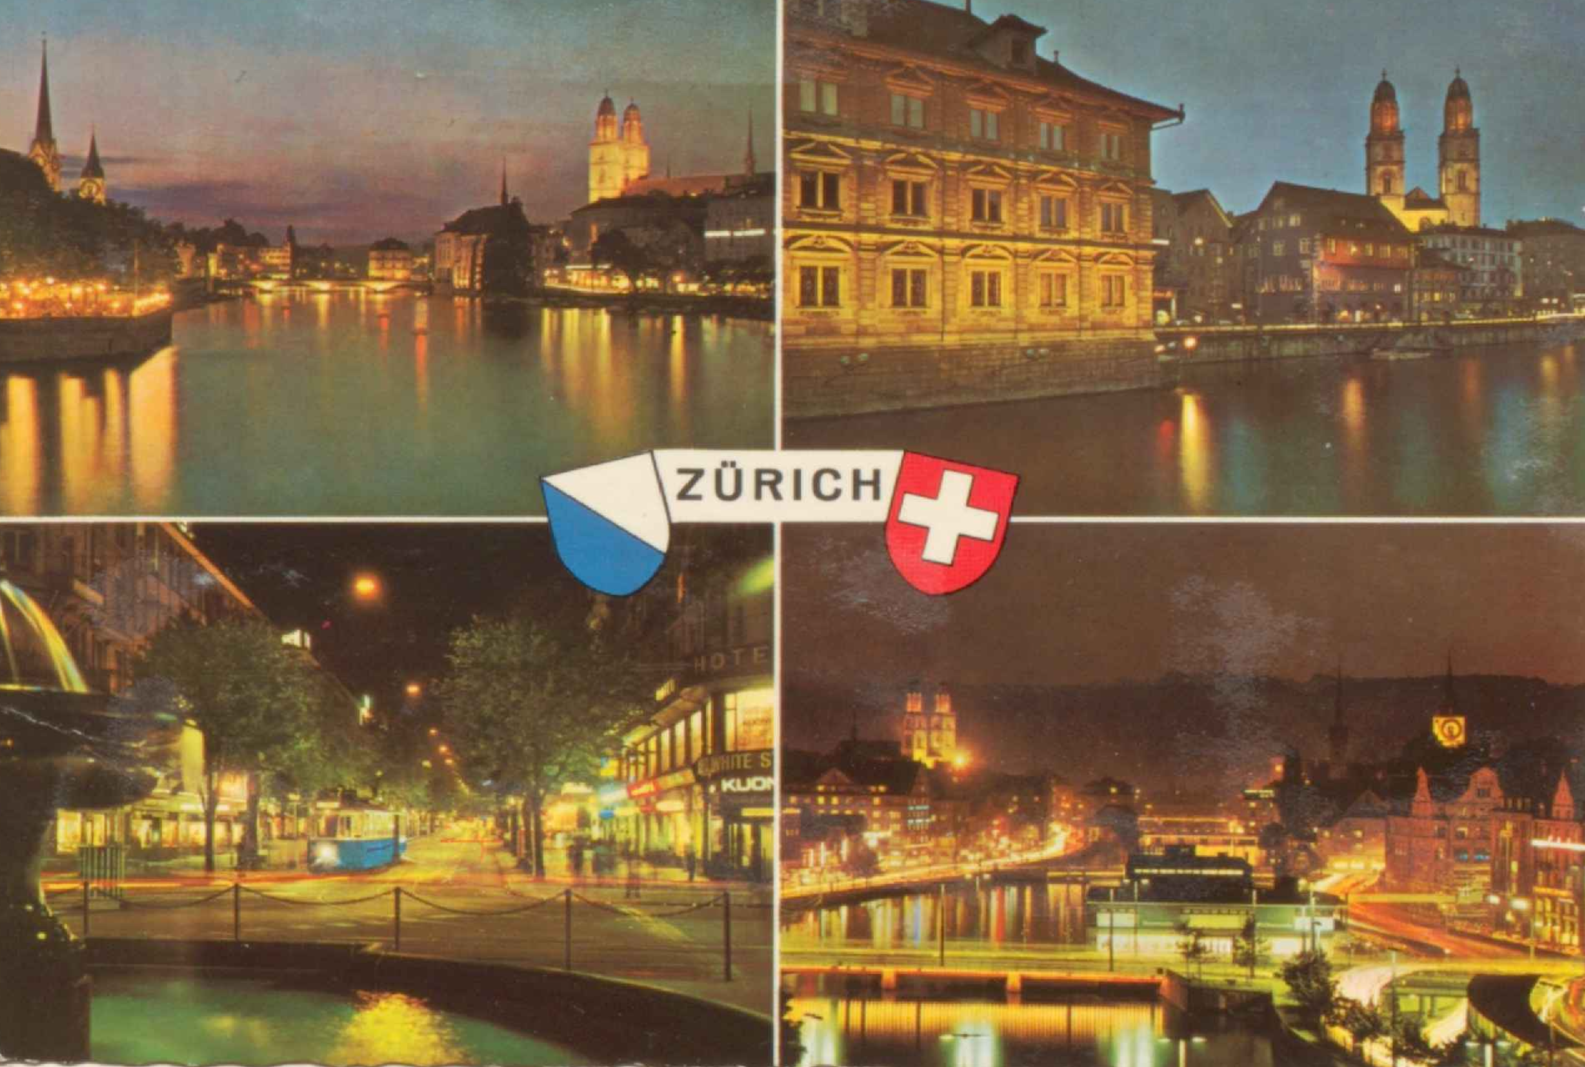
\includegraphics[width=\textwidth, height=\textheight, keepaspectratio]{250-a-curych}
\caption{ V městě Curychu ve Švýcarsku žije vnuk Františky Barthové, rozené Prusíkové}
\label{fig:250-a-curych}
\end{figure}

             \begin{figure}
\centering
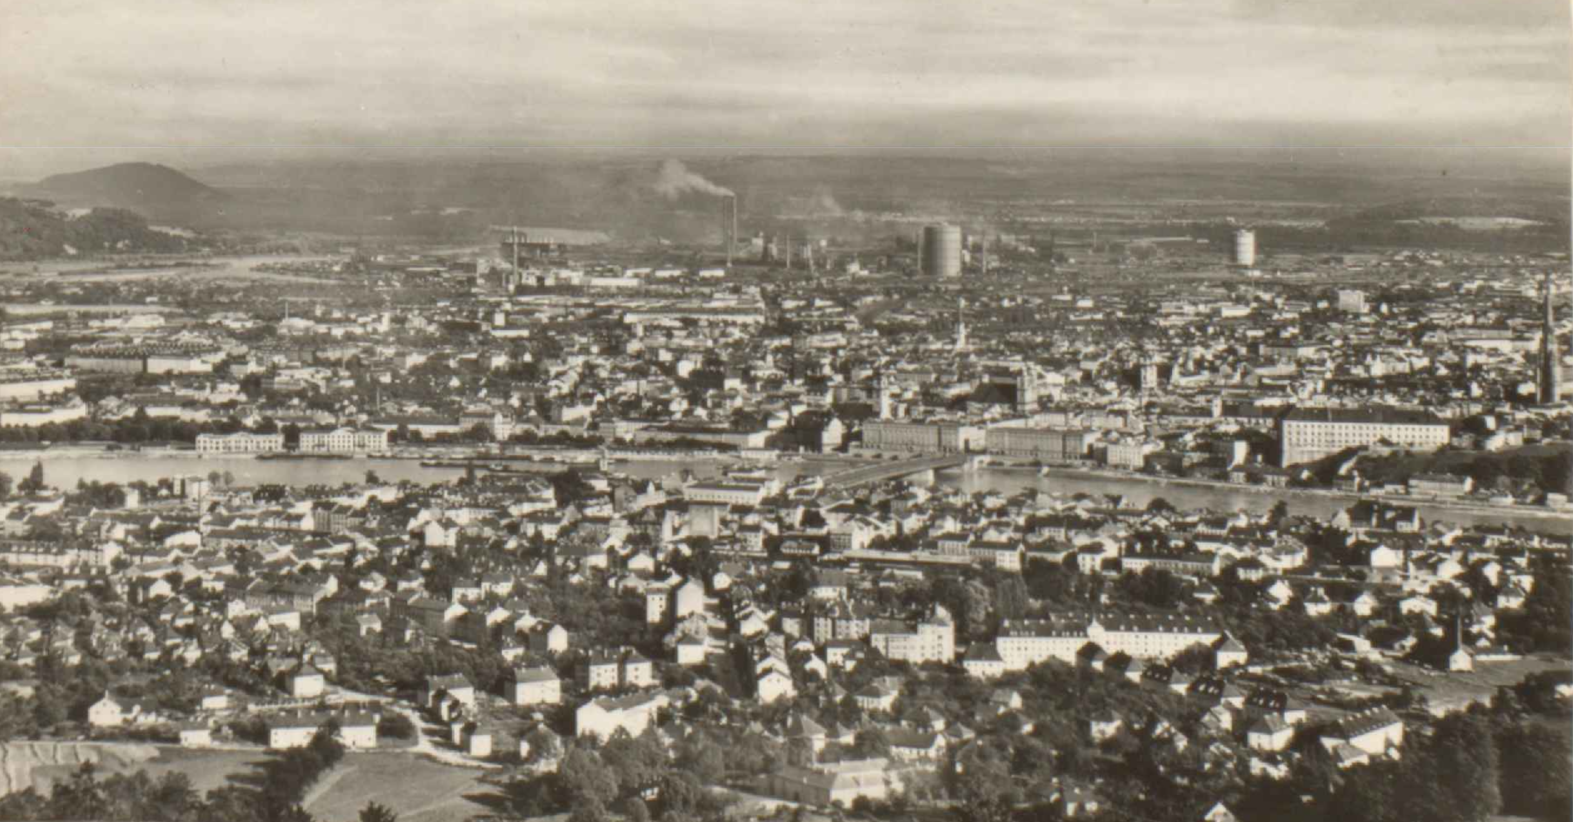
\includegraphics[width=\textwidth, height=\textheight, keepaspectratio]{250-b-rakousko_linec}
\caption{V Linci v Rakousku bydlí dcera Františky Barthové ze Žatce, narozená v Plasích}
\label{fig:250-b-rakousko_linec}
\end{figure}

% str 216 @ 251
Třetím dítětem Růženy Barthové, provdané Hübnerové je dcera Friederika nar. 26. 6. 1943. Nebyly jí ani dva roky, když prožila s matkou, a sourozenci květnovou revoluci v Praze. Nemají na tuto dobu dobré vzpomínky. Friederika je dnes provdaná Mascheková v Linci. Má dceru Ulriku, narozenou 15. 4. 1968.

Popsali jsme tímto osudy všech potomků Frantiska Prusíka, narozeného v roce 1824 ve Stražišti. Zvláště u těch, kteří se poněmčili a těch je naprostá většina, a kteří ještě žili před druhou světovou válkou a za ní v Čechách jsou osudy velmi pohnuté. Přinesla to všechno sebou válka a zjevy, které ji doprovázely. Postihly těžce nejen český národ, ale i mnoho příslušníků německé národnosti, kteří často se nijak neprovinili, než že patřili k německé národnosti.

Dalším dítětem zednického mistra Vojtěcha Prusíka ve Stražišti, který se tam narodil na sklonku panování císaře Josefa II., byl syn Antonín. Narodil se 12. 1. 1826. Stal se obuvníkem a měl poměrně nuzný život. Když zestárl dělal poštovního poslíčka a denně chodil ze Žíhle do Stražistě, což byla opravdu pěkná "procházka“. Antonín Prusík oženil se po prvé s Annou Soukupovou nar. v roce 1847 ve Stražišti. Ta však zemřela 10. 5. 1873 po dítěti. Byl již tedy Antonín Prusík dosti starý 46 letý, když se ženil po prvé. Děcko také zemřelo. Antonín Prusík oženil se pak znovu s Annou Fryčkovou nar. 20. 2. 1850 v Mladoticích. Měli spolu dva syny a tři dcery. Život měli neveselý, byla to jen sama dřina a peněz málo. Když nešlo řemeslo, sloužilo se u sedláků, v lese a pod. Po smrti Antonína Prusíka 28. 12. 1900 ve Stražišti, odstěhovala se vdova ke své provdané dceři Valentýně do Manětína a tam zemřela 28. 7. 1912.

\section{První Prusík v Kanadě}
Nejstarším dítětem Antonína Prusíka a Anny roz. Fryčkové byl syn Bedřich. Narodil se 2. 3. 1876 ve Stražišti. Vychodil pětitřídku ve Stražišti a od dětství musel pomáhat rodičům, kteří neměli na růžích ustláno. Naučil se však slušně německy, vždyť kousek za vesnicí Stražištěm byly již německé obce. Bedřich Prusík odešel pak ke Ka­dani a k Žatci a tam sloužil u sedláků, což přece jen byl poněkud lepší život než doma. Na začátku tohoto století a ovšem již před tím, vznikla velká touha hledati štěstí za mořem. Tomuto lákadlu neodolal ani Bedřich Prusík. Všechny své malé úspory věnoval na cestu do Ham­burku a přes moře do Kanady. V roce 1901 přistál v místě zvaném Glace Bay. Je to přístavní městečko na Atlantickém oceánu v provincii Nova Scotia v Kanadě. Blízko tohoto místa byly velké doly a uhlí se vlastně dolovalo až pod mořem. Bedřich Prusík stal se horníkem a doufal, že zde nalezne konečně své životní štěstí. Tento sen se mu však nevyplnil. Každý, kdo jel za velkou louži, nezbohatl. Nejdříve pracoval Bedřich Prusík v městě Sydney Mines. To bylo blízko přístavu, kde vstoupil poprvé na půdu Kanady. Zpočátku se mu dařilo dobře, postavil si i domek a zatoužil pak také po vlastním rodinném krbu.V roce 1907 vrátil se do Čech a odtud si přivezl ženu. Byla to Marie Čechová, nar. 31. 7. 1880 v Chrašťovících. Bedřich se s ní
% str 217 @ 253
znal již od mladých let, vždyť Stražiště a Chrašťovice jsou sousední obce. Když se Bedřich se svou manželkou vracel do Kanady, nalákal k odjezdu ještě svého bratra Františka. Usadil se pak opět v Sydney Mines a tam pracoval v dolech. Zde se jim narodily dvě děti. Marie 4. 10. 1908 a Bedřich 29. 1. 1910.

% str 216+1 @ 252
% TODO foto

% str 217 @ 253 (pokr.)
Marie je provdaná za dělníka Viléma Nicholsona a bydlí v Sydney Mines PO BOX 588. Marie, jako ostatní její tři sourozenci rozumí česky, ale nedovedou již číst a psát v rodné řeči svých rodičů. Marie Nicholsonová roz. Prusíková má dva syny. Starší je Hugo nar. 18. 6. 1928, bydlí ve státě Ontario v Kanadě v městečku Hagersville. Je dělníkem. Má tři děti. Dcerku Annu nar. 16. 6. 1951, synka Ericha nar. 15. 2. 1953 a další dceru Alžbětu nar. 21. 9. 1956. Druhý syn je Vilém Nicholson nar. 30. 7. 1929. Je také dělníkem. Bydlí v městě Toronto 227, Symington Avenue. Má jednoho synka Viléma, nar. 15. 12. 1958.

Druhé dítě narozené manželům Prusíkovým v Sydney Mines, byl syn Bedřich. Narodil se 29. 1. 1910 a bydlí také v místě kde se narodil, 225 Main Street. Jeho manželkou je Berta Ramseyová nar. v Kanadě 14. 3. 1915. Bedřich Prusík pracuje také v dolech jako kdysi jeho otec. Je bezdětný.

Když se Bedřichovi Prusíkovi přestala zamlouvat těžká práce v dolech, což se také začalo projevovat na jeho zdraví, odstěhoval se s dvěma dětmi v roce 1912 daleko na západ Kanady do státu Alberta, blíže městečka Wetoskiwin. Tam pracoval Bedřich Prusík na farmě a později ve mlýně a pobyl tam čtyři leta. Těžký život to byl také, ale přece jen na vzduchu a ne v podzemí. Na tomto kanadském venkově, vzdáleném 4.000 km od Atlantického oceánu narodilo se další dítě a to Anna. Bylo to 29. 4. 1915. Dnes žije Anna jako provdaná Sampsonová v městě Scarborough na břehu velkého kanadského jezera ve státě Ontario. Její adresa je Bertha Avenue 63. Anna Sampsonová rozená Prusíková je bezdětná. V roce 1916 odstěhoval se Bedřich Prusík se svými třemi dětmi a manželkou do města Lethbridge v západní Albertě. Tam se narodil druhý syn Jaroslav 8. 4. 1919. Po anglicku říká se Jerry. Jerry Prusík je dosud svobodný a žije se svou matkou v Sydney Mines a pracuje v průmyslu rybích konzerv. Matka jeho vždy tak pracovitá, hledá mu stále nevěstu v Čechách, ale dosud se žádná "partie" nenašla.

Bedřich Prusík vrátil se v roce 1920 opět do Sydney Mines a pracoval tam ještě krátce v dolech. Brzy pak onemocněl tuberkulosou a zemřel 11. 2. 1921. Zvláštní štěstí za velkou louží nenašel, ale naopak těžkou práci a brzkou smrt.

Druhým dítětem Antonína Prusíka ve Stražišti byla dcera Valentina. Narodila se 11. 2. 1878, vdala za malozemědělce Leopolda Grüna  do Manětína. Za svobodna sloužila asi tři roky u sedláka Vojtěcha Prusíka ve Výrově. Tehdy o sobě nevěděli, že jsou vzájemně spřízněni. Bylo to v letech 1895 – 1898. Valentina Grünová rozená Prusíková měla dvě děti. Je to dcera Albína nar. 31. l0. 1909. Zůstala svobodná a pracuje jako dělnice u lesní správy. Bydlí
% str 218 @ 254
v Manětíné č. 58. U ní zemřela matka 12. 10. 1960. Druhý byl syn Václav Grün nar. 13. 9. 1913. Pracuje u státního statku v Nečtinách a bydlí v Leopoldově č. 16 u Nečtin. Několik let tam s ním žila matka, dnes již mrtvá. Je svobodný.

Druhým synem Antonína Prusíka byl František. Narodil se 11. 5. 1886 ve Stražišti. Také on měl těžký život. Chodil do školy ve Stražišti a v tamním výstavném kostele sv. Martina tři roky ministroval. Dnes vzpomíná ještě jak tam zvoníval na tři zvony, jejichž hlas byl daleko do kraje slyšitelný. Zvony z tohoto kostela hlásaly celému, širému kraji 11. listopadu 1918 konec světové války.

František Prusík až do roku 1907 vlastně dělal podruha. Nebylo tedy divu, ze se dal přemluvit svým bratrem, který žil již od roku 1901 v Kanadě, a odjel s ním za moře. Dne 10. prosince 1907 přijel, jak často vtipně říká, do té "zaslíbené" země. Ale ani on tam žádné zvláštní štěstí nenašel. Velký kus života strávil v té zmrzlé Kanadě pod zemí a mnohdy byl ten kousek chleba vezdejšího opravdu v potu tváře dobytý. František Prusík měl všude domov, kde si mohl pověsit klobouk neb čepici a kde našel práci. Nejdříve byl také horníkem v Sydney Mines, ale brzy odjel daleko do státu Alberta, kde byly lákavější podmínky. Pracoval v dolech až do roku 1935 kdy se při výbuchu uhelných plynů zázrakem zachránil, ale památku po této katastrofě má dodnes. Při explosi přišlo tenkrát o život 16 horníků a z toho 3 Češi. František Prusík, věrný to Čech, nikdy svou řeč nezapomněl a přesto, že dnes žije v domově důchodců mezi lidmi jiných národností zcela sám,  píše dobře česky a často opakuje slova "Kdo se za svůj jazyk stydí, hoden potupy všech lidí!"

Když jsme tohoto kanadského Prusíka konečné nalezli a popsali mu původ starého našeho rodu i význam odpově­děl takto: "Jsem rád, že patřím mezi rod Prusíků, za který se nikdo stydět nemusí. Všichni jsme ovšem tak jako někteří z tohoto rodu nevynikli. Nadání by bylo bývalo u mnohých, ale k lepšímu postupu vzdělání chyběly finance. Ta nešťastná chudoba, ta mnoho zla provedla a mnohý chudý za rakouské vlády se narodil a chudý zemřel. Nebýt však těch chudých otroků hloupých, jak je chytrá­ci nazývají, zašli by ti chytráci hladem. Žiju zde již přes 60 let, ale jak vidím, jméno Prusík brzy bude zde všude v Americe a Kanadě jen podle jména a již ne podle českého jazyka a národnosti."

František Prusík žije dnes v městě Pincher Creek Crest View Lodge ve státě Alberta v Kanadě. Škoda, že tak věrných Čechů žije již málo za mořem. František Prusík zůstal svobodný a rád si dopisuje se svými příbuznými ve své vlasti. František Prusík zemřel v opuštěnosti dne 9. května 1968 a byl pohřben na hřbitůvku v Fincher Creek ve státě Alberta v Kanadě právě v den svých 82. narozenin dne 11. května 1968.

% str 219 @ 255
Druhou dcerou Antonína Prusíka ze Stražiště byla Marie. Narodila se 14. 5. 1880 ve Stražišti. Sloužila u obchodníka Lőbla v Kožlanech a tam se seznámila s tkadlecem Oldřichem Kratochvílem. Za toho se v roce 1909 provdala. Její syn byl Adolf  narozený 30. 9. 1910, který dnes pracuje v průmyslu v Žatci. Bydlí v ulici Boženy Němcové 29. Adolf Kratochvíl má dvě dcery. Milena nar. 28. 9. 1940 je provdaná Ždychová a bydli s rodiči. Má syna Pavla nar. 6. 4. 1964. Milena Ždychová má též dceru Ivettu, narozenou 23. 11. 1968. Druhá je Libuše narozená 6. 3. 1946 a je provdaná Vávrová v Klášterci nad Ohří, Sídliště Miřetice č. 406. Má synka Aleše nar. 2. 6. 1968.

Druhým dítětem Marie Kratochvílové roz. Prusíkové byla dcera Marie. Narodila se 25. 9. 1913 a bydlí dnes v Radonicích č. 172 u Kadaně. Má dceru Alenu nar. 8. 6. 1940. Je provdaná Prchalová a žije v Jincích č. 70 u Příbrami. Má dcerku. Alenu nar. 6. 3. 1966. Dále je Miroslav Došek, jak byla jeho matka provdaná, který se narodil 23. 3. 1948. Marie Kratochvílová roz. Prusíková zemřela po zápalu plic 30. 3. 1917 v Plzni.

Třetí dcerou Antonína Prusíka byla a Albína. Narodila se 19. 6. 1883 ve Stražišti. Vdala se za krejčího Jana Pleinera do Manětína. Jako její sestra Marie, zemřela i ona mladá ve 34 letech dne 10. 9. 1917. Albína Pleinerová roz. Prusíková měla jedinou dceru Marii. Ta se narodila 14. 3. 1914 v Manětíně. Je dnes provdaná Kučerová a bydlí v Praze 1, Karlova 48. Má dva syny, Františka nar. 1. 8. 1943 a Jiřího nar. 30. 1. 1947. Marie Kučerová nezapomíná na svoje rodiště a celý rodný kraj jako je Manětín, Stražiště nebo Plasy.

Kolem roku 1788 přišel z Plas do Stražiště první Prusík a to Adam. V roce 1900 zemřel ve Stražišti poslední Prusík a to Antonín, jeho vnuk. Byl tam tedy náš rod 112 let. Potomci jejich žijí dnes s naším jménem i mno­ha jinými u nás a v cizích zemích. Měli přepestré osu­dy, někteří z nich vynikli, ale mnozí také musili si svou skývu chleba dobývati velmi těžce. Mnoha z nich je posledním domovem idylický hřbitůvek stražištský, ale četní složili své kosti daleko od svého rodiště, za mořem, v Rakousku, Německu a jinde.

Třetím synem Vojtěcha Prusíka, zednického mistra ve Stražišti, byl Josef. Narodil se 7. 3. 1828. Vyučil se krejčovině v Kralovicích a mluvil dobře německy jako česky, vždyť otec byl Čech a matka Němka. Odešel pak brzy do Vidné, tam měl svou krejčovskou dílnu a v době prusko-rakouské války se oženil s Eleonorou Petrův, která se narodila v roce 1831 v Nových Benátkách nad Jizerou. Poznali se ve Vídni, kde tehdy žilo již velké množství Čechů. Krejčí Josef Prusík však dlouho nežil, zemřel ve Vídni 23. 3. 1872. Jeho manželka zemřela v roce 1891. Měli jediného syna Karla. Ten byl již úplným Němcem. Narodil se ve Vídni 23. 9. 1867. Vyučil se truhlářem a čalouníkem. Zvláštních zásluh si dobyl tím, že byl
% str 220 @ 256
zakladatelem několika spolků pro ochranu mládeže. V této činnosti vyvíjel velkou aktivitu a zachránil od špatného osudu mnoho mladých lidí. Manželkou jeho byla Marie Weberová nar. 1. 2. 1868 v Mikulášovicích ve Slezsku. Karel Prusík zemřel ve Vídni za druhé světové války 23. 4. 1943. Jeho žena Marie dokončila svůj život za šest let po něm, 23. 3. 1949. Oba jsou pohřbeni ve Vídni. Měli jediného syna Karla, který se narodil  19. 5. 1896 ve Vídni. Tento Karel Prusík později proslavil naše jméno v celém světě. Povíme Vám jak.

\section{Jak se jméno Prusík stalo pojmem}
Když někdo bydlí v mansardě sotva ví, proč se ta místnost v podkroví tak jmenuje. Původně tak začal stavět francouzský stavitel Mansarde. Bývá-li v řecko-římském zápase použito nelsona, sotva kdo pomyslí, že prvně tímto způsobem začal zápasiti Američan Nelson. Zrovna tak si málokdo uvědomí, že dělový náboj šrapnel je pojmenován podle anglického generála Shrapnella a málokdo tuší, že slovo brajgl je odvozeno od slavného malíře Breughela, jehož obrazy představuji obyčejně rušná posvícení venkovská, lidové rvačky a podobné pohnuté události. Horolezci v celém světe znají záchranný uzel "prusík" a také asi sotva vědí, že jeho vynálezcem byl člen našeho rodu Dr. Karel Prusík z Vídně.

Karel Prusík studoval na universitě ve Vídni filosofii a později dějiny hudby a hudbu samotnou. V roce 1924 získal v tomto oboru doktorát na vídenské universitě a brzy pak stal se profesorem na vídenské konservatoři. Již jako patnáctiletý chlapec konal dlouhé únavné pochody do hor a když mu bylo l8 let, slezl již některé těžké alpské vrcholy v pohoří Gesäuse a v Dolomitech. V první světové válce byl již na alpské frontě jako poručík, utrpěl tam zranění a omrzliny a léčil se z nich také pak v Praze ve vojenské nemocnici na Hradčanech. Podle jeho slov byla to jediná návštěva jeho v Čechách v roce 1916, ačkoliv jeho rod odtud vzešel.

Po první světové válce věnoval se Dr. Karel Prusík plnou silou svým dvěma láskám. Horolezectví a hudbě. Jistě je to krásná symbiosa těchto dvou činností. Být vysoko v horách sám a nerušen a při tom myslet na vznešenou hudbu, která tak povznáší člověka! Pro tuto svou vášeň se Karel Prusík dlouho neženil. Ve svém životě vykonal asi 70 prvovýstupů na různé vrcholy v Alpách rakouských, ale i v Jugoslávii na severní stěnu Triglavu, ve Vysokých Tatrách a v rumunských Karpatech. Karel Prusík byl jeden z prvních horolezců, který učil jak možno použíti ve velehorách lyží. V sedle mezi Gross Glocknerem a Hochtorem, kde také provedl některé prvovýstupy, je po něm pojmenovaná velehorská rokle.

Věhlas jeho mezi horolezci stoupl od roku 1931, kdy vynalezl záchranný uzel nazvaný později jeho jménem. V prvních
% str 221 @ 258
dobách se uzlu říkalo Prusíkův uzel.  Co to je? Používá se hlavně pro smyčky ze šňůry, které se upevňují na laně. Nejsou-li správné zatíženy, snadno se po laně posunují. Když je zatížíme správně, nepohnou se ani o milimetr. Obtočíme-li smyčku jednou vznikne jednoduchý Prusíkův uzel, dvojitým obtočením dvojitý prusík. Platí zde zásada, že prusík drží tím více, čím větší je rozdíl průměru lana a smyčky. Známe tkalcovský uzel, lodní smyčku, farmářskou smyčku, dračí smyčku, které se mezinárodně říká "Bowline", rybářskou spojku, plochou spojku, nebo tzv. ambulantní uzel a také všude ve světě prusíka. Tak se stalo na­še jméno všeobecně vžitým pojmem.

% str 220+1 @ 257
\begin{figure}
\centering
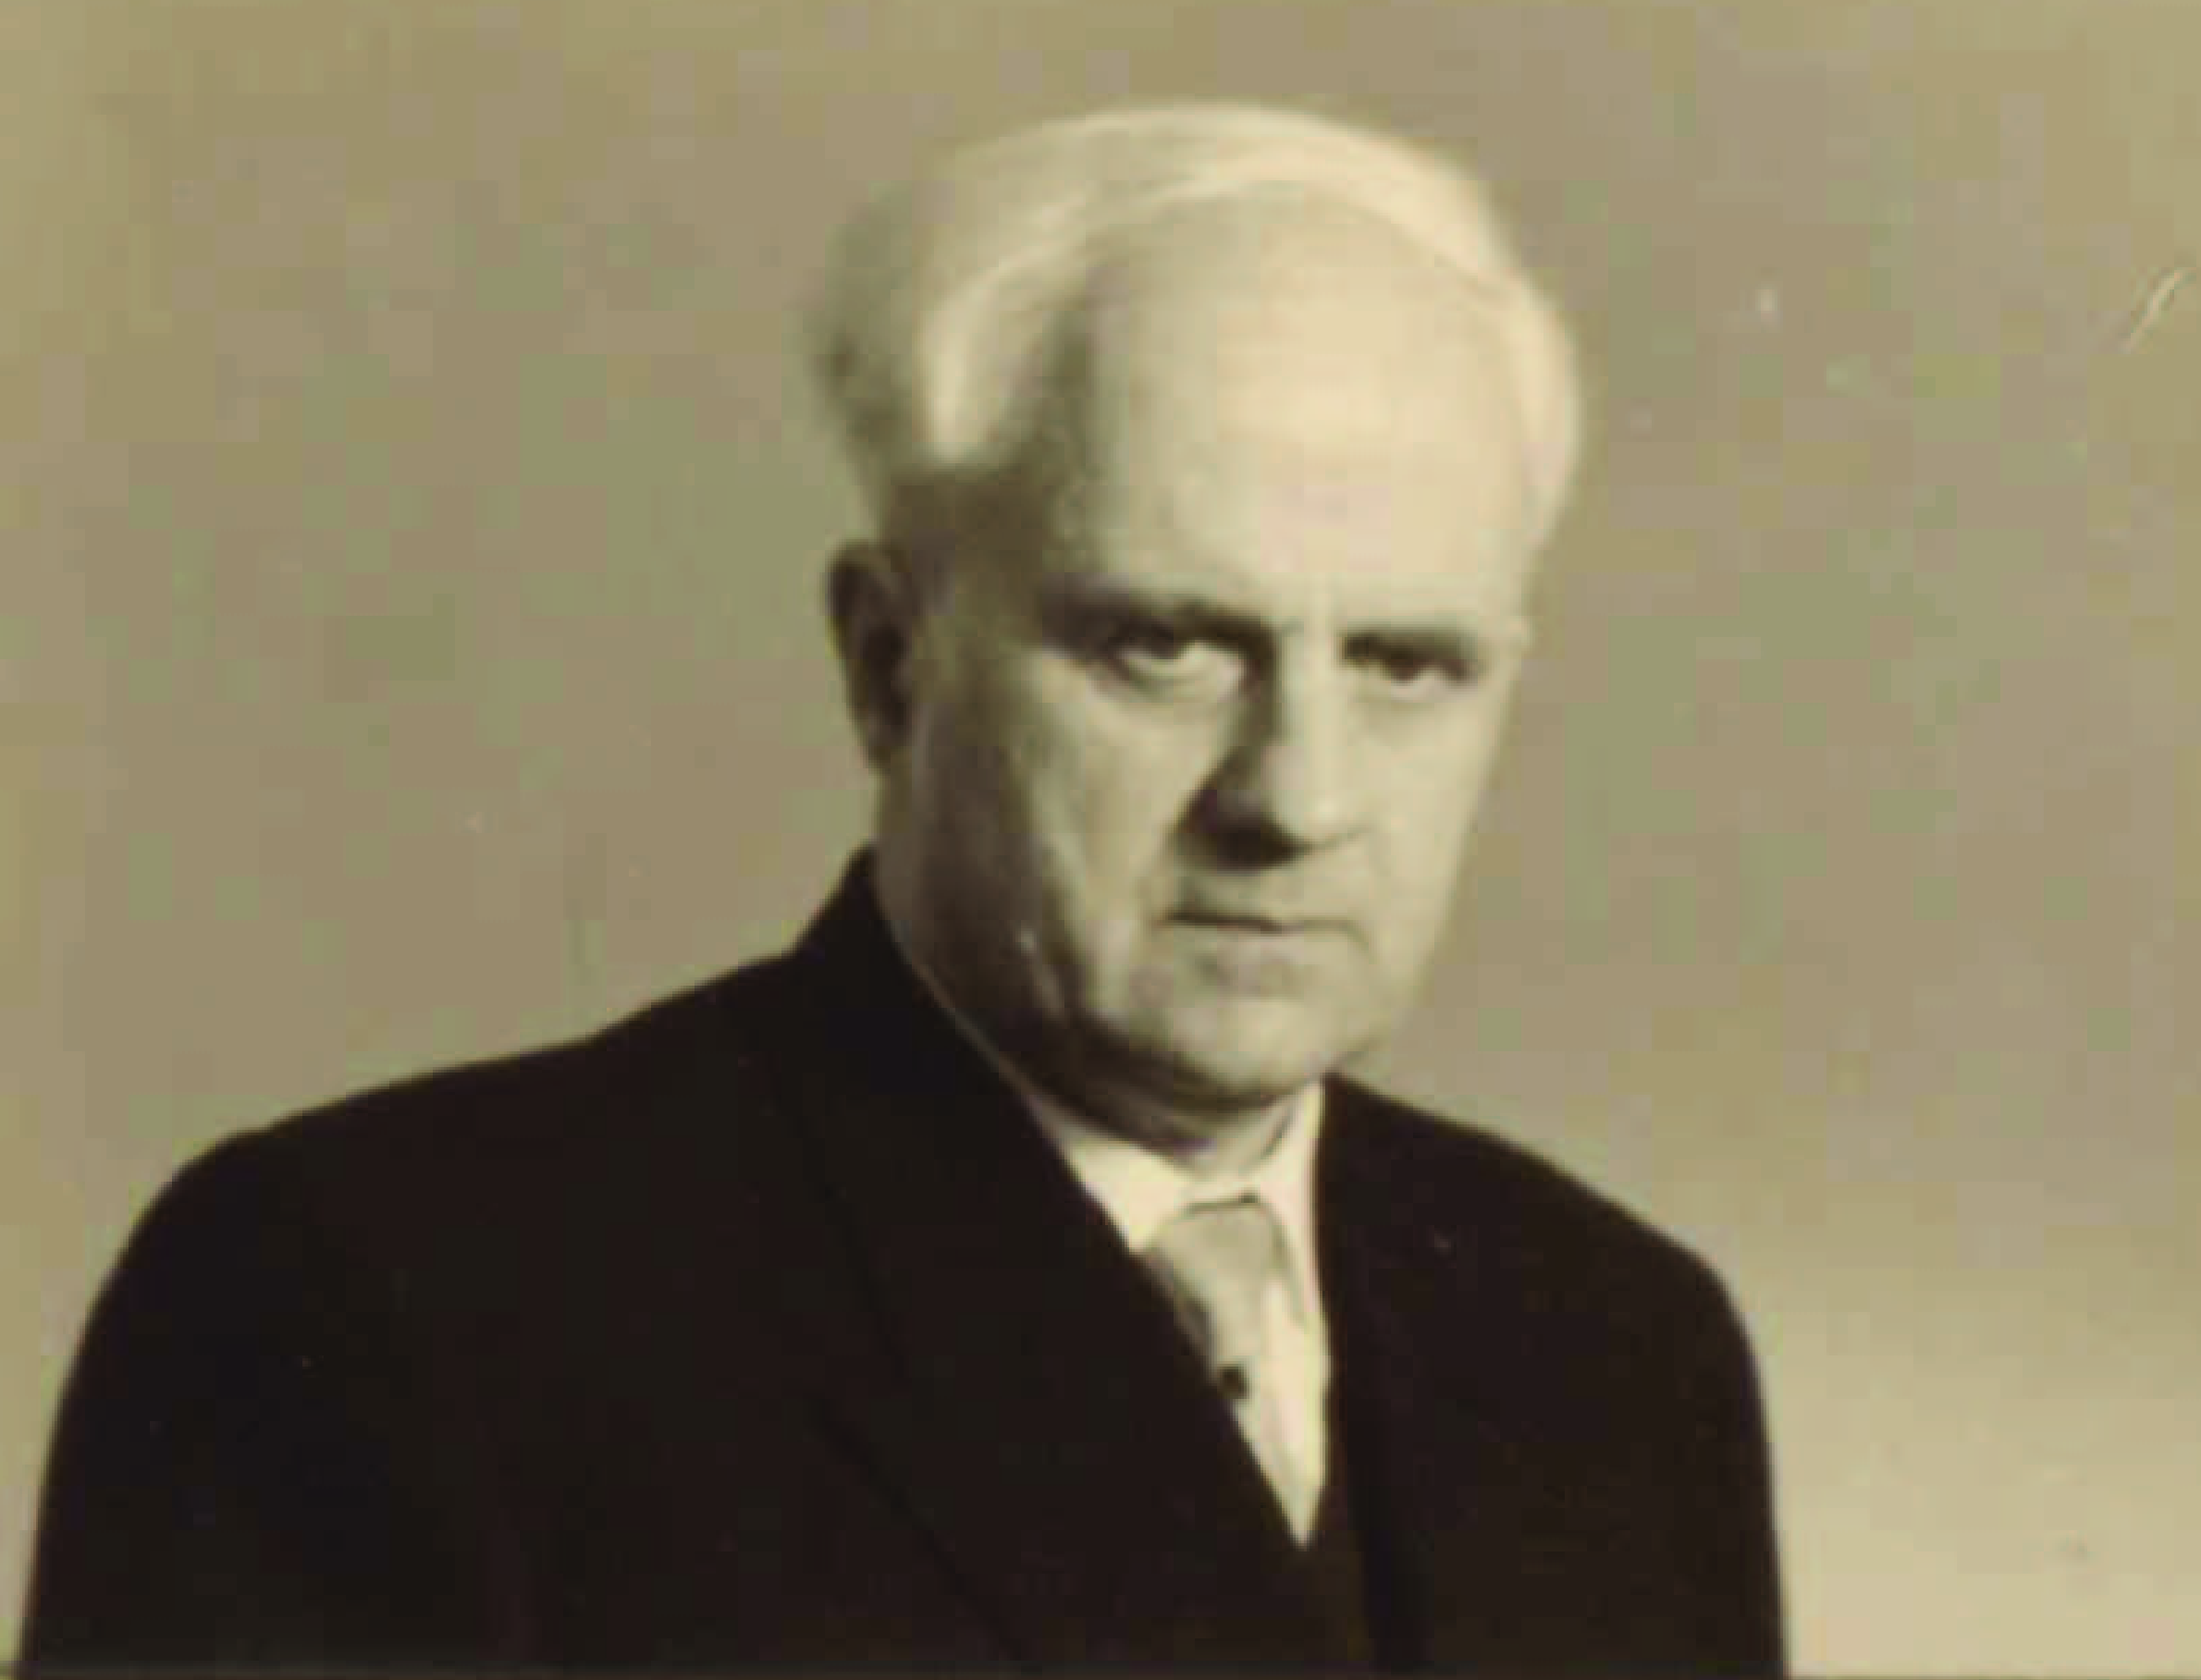
\includegraphics[width=\textwidth, height=\textheight, keepaspectratio]{257-a-prof_dr_karel-prusik}
\caption{Profesor dr. Karel Prusík, horolezec, profesor na vídeňské konservatoři, vynálezce světově proslulého horolezeckého záchranného uzlu (1896 – 1961)}
\label{fig:257-a-prof_dr_karel-prusik}
\end{figure}

             \begin{figure}
\centering
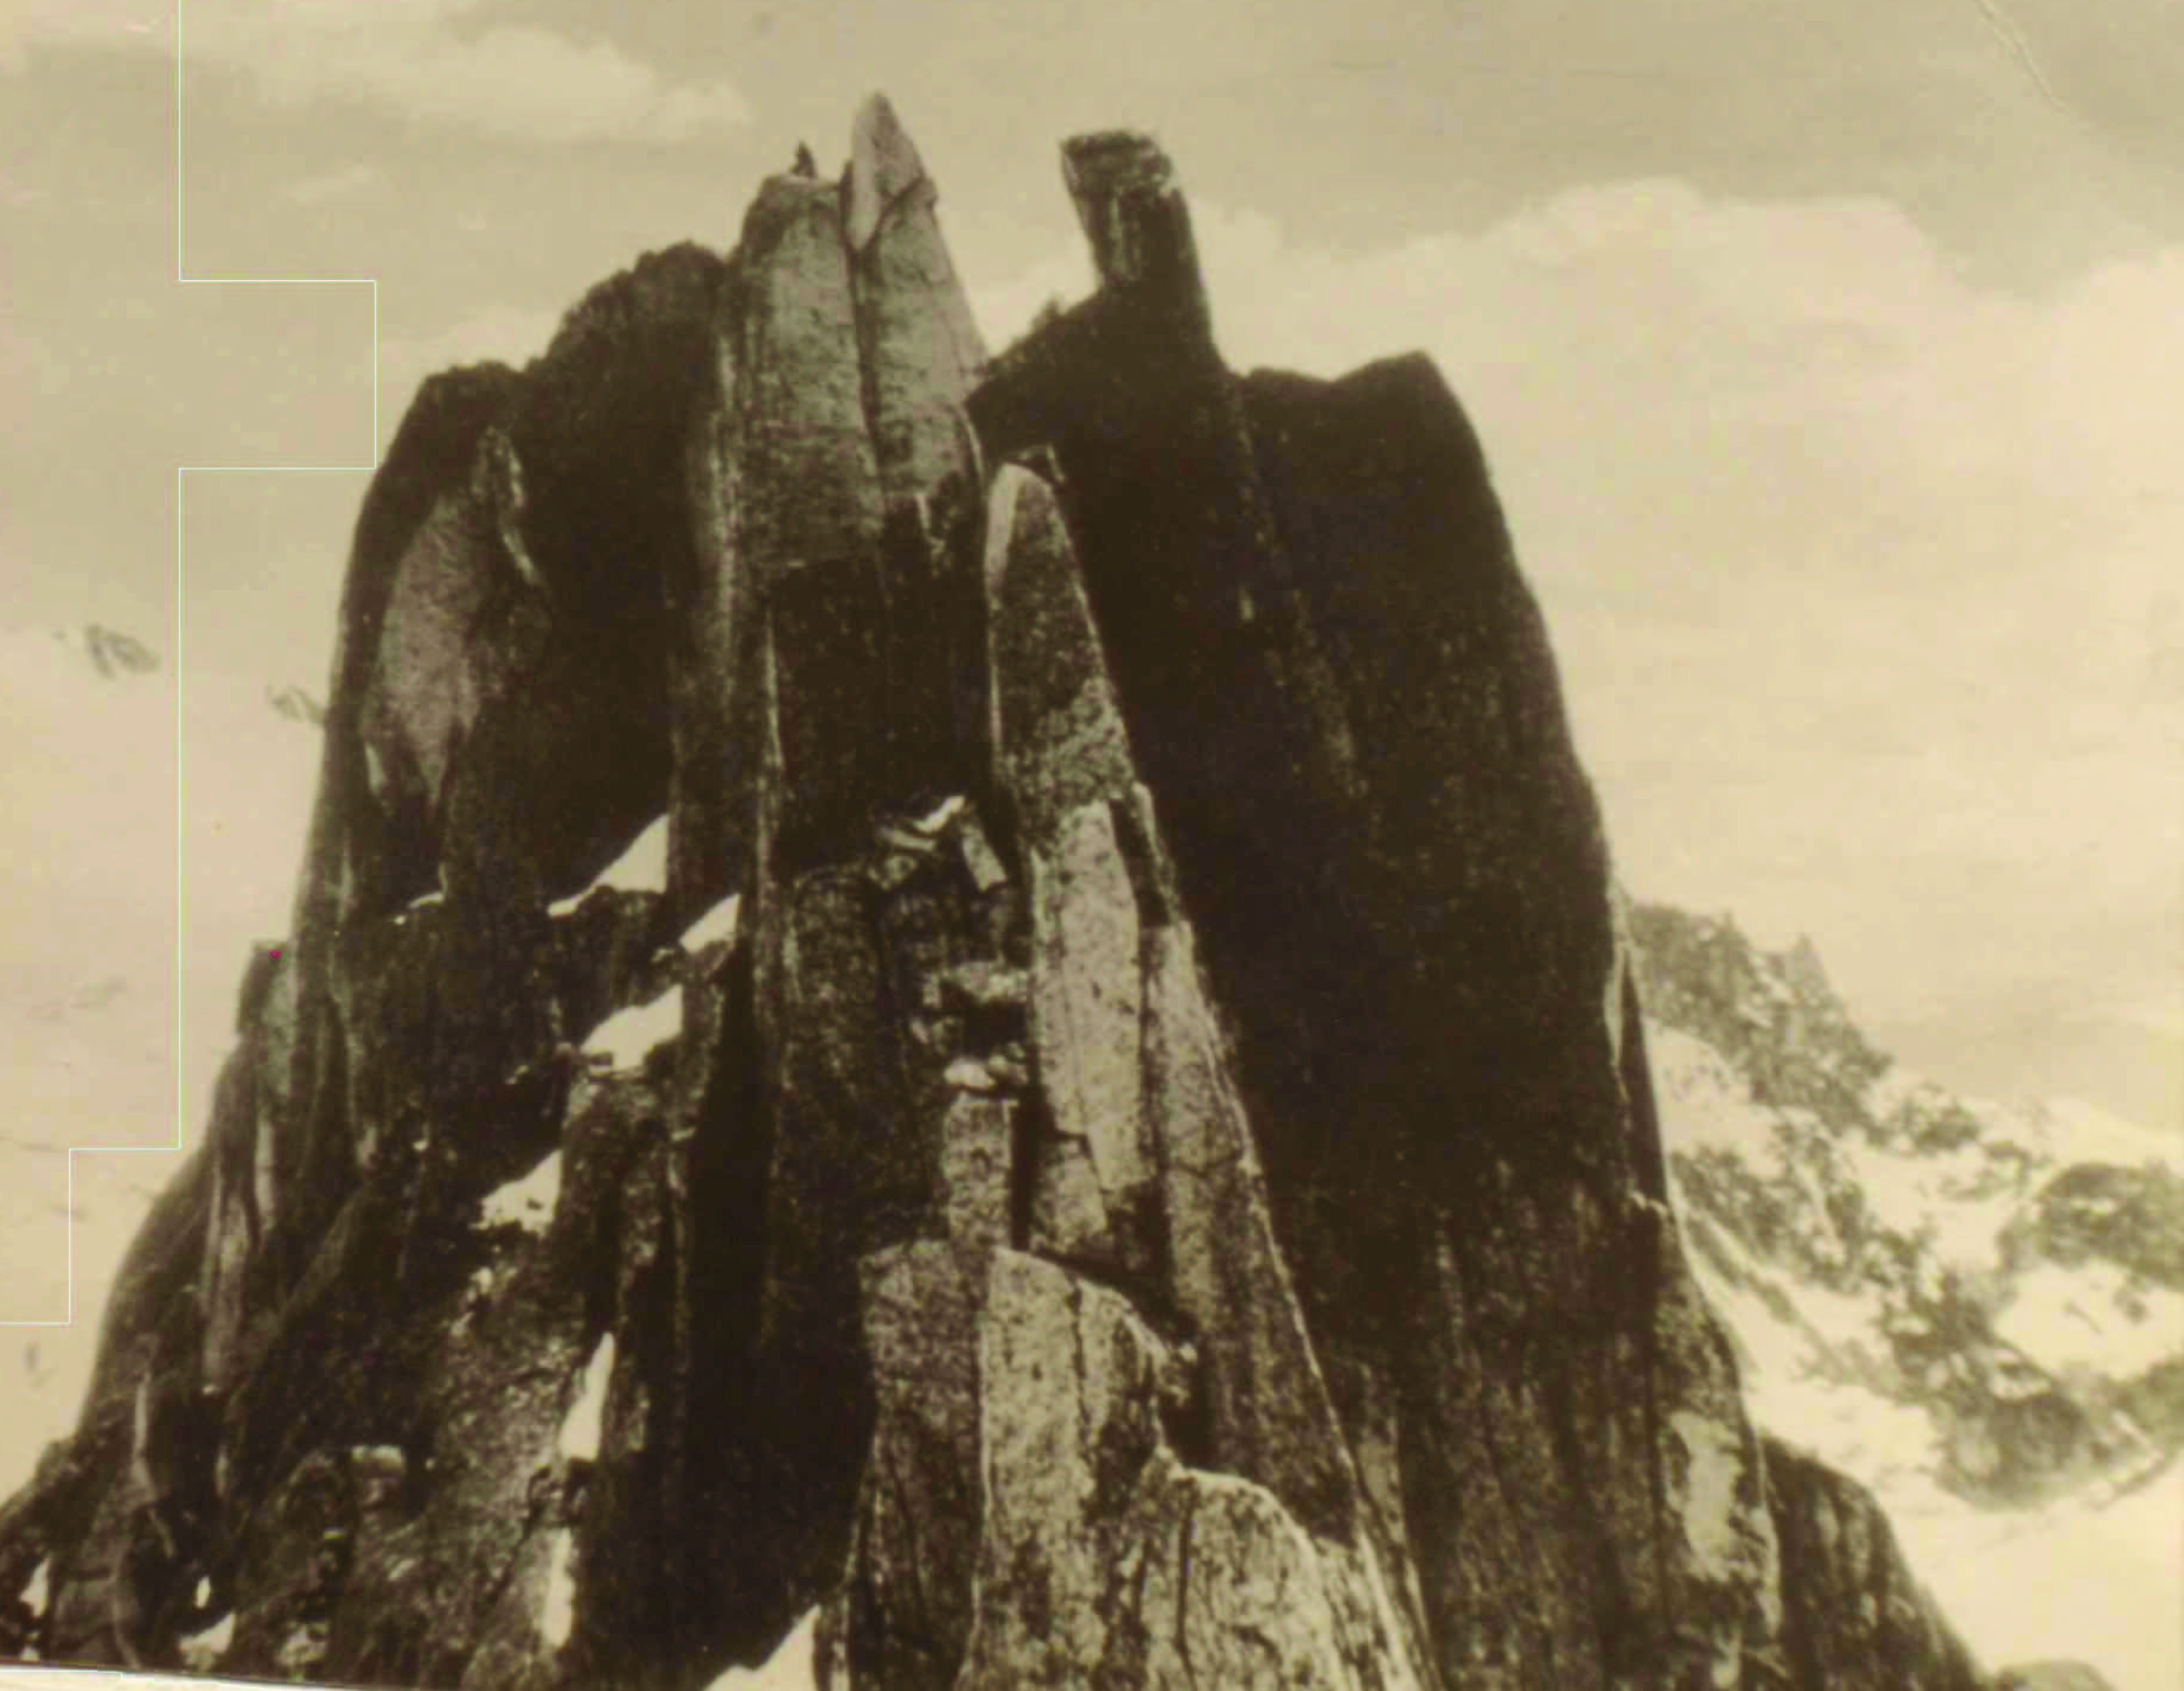
\includegraphics[width=\textwidth, height=\textheight, keepaspectratio]{257-b-prusikova_hora}
\caption{Prusíkova hora „Prusik Peak“ ve Skalistých horách ve státě Washington v USA}
\label{fig:257-b-prusikova_hora}
\end{figure}

% str 221 @ 258 (pokr.)
Za své zásluhy dostal Dr. Karel Prusík nejvyšší řád Rakouské republiky v roce 196l, nedlouho před smrtí. Od roku 1950 stal se presidentem sdružených rakouských alpských klubů a byl také čestným členem Rakouského alpského klubu, kteréžto pocty se dostalo jen několika jednotlivcem. Jeho uzel zachránil tisícům život v horách.

Jako hudebník a vychovatel na vídenské konservatoři a na městské hudební škole v Perchtolsdorfu, kde bydlel, věnoval největší zájem hře na kytaru. Na gramofonových deskách i v notovém vydání je zachyceno asi deset jeho komposic, zvláště písní opěvujících hory a staré lidové zvyky. Karel Prusík nevyučoval jen hře na kytaře, ale i na housle a jiné hudební nástroje. Napsal také kromě mnoha básní i román Faust a hora. Z jeho podnětu byl zřízen pamětní hřbitov obětem hor blíže kláštera Admont v romantickém údolí řeky Emže pod alpskými velikány.

Když se Dr. Karel Prusík vrátil z druhé světové války, oženil se pak brzy s Annou Rinckovou narozenou 13. 12. 1900 v Heilbrunnu u Stuttgartu. Neměli však již spolu děti.

Máme-li prusíkovský uzel, máme také naši horu. V roce 1948 byl poprvé slezen dvěma Američany vrchol hory v pohoří Cashmere Crags, což je součást severoamerických hor ve státě Washington, blíže  Tichého oceánu v USA. Tito horolezci použili uzlu prusíka a po jeho vynálezci nazvali tuto horu Prusik Peak. Tehdy ani nevěděli, že vynálezce Dr. Karel Prusík žije v Rakousku. Jen v Rakousku je dnes asi 250 tisíc horolezců a také u nás a ve všech zemích, kde mají hory, počet horolezců rychle roste. Nebezpečný, ale krásný tento sport stal se módou dneška. Tím proniká i dále naše jméno do světa.

Když se konal v říjnu 1958 první, sjezd našeho rodu v Praze, měl Dr. Karel Prusík vážný úmysl zúčastniti se této rodové schůzky. V té době však již trochu churavěl a 28. 5. 1961 podlehl zákeřné rakovině prostaty v Perchtolsdorfu u Vídně, v bytě, z jehož oken viděl na své milované hory. Dr. Karel Prusík patří jistě k významným členům našeho rodu. Vdova po něm Anna Prusíková bydlí v Perchtolsdorfu, Brunnergasse 1.

% str 222 @ 259
Dalším dítětem Vojtěcha Prusíka ve Stražišti byla dcera Anna. Narodila se 25. 7. 1830 ve Stražišti. Provdala se 24. 11. 1857 za hajného Jana Monsé. Děd jeho přišel po francouzské revoluci do Čech. Muž Anny Prusíkové Monsé působil na hájovně Černá jáma u Kaznějova, která dnes již neexistuje. Také byl v Lomanech, což vše náleželo k panství Metternichově v Plasích. Anna Monséová roz. Prusíková měla sedm dětí a z toho tragicky zemřely na záškrt v jednom měsíci čtyři. Byl to Karel nar. 23. 7. l859, který zemřel 16. 1. 1879. Dále Rudolf nar. 27. 3. 1863 a zemřel 24. 1. 1879. Pak to byl Josef Monsé nar. 13. 10. 1864, který zemřel 10. 1. 1879 a jejich sestra Anna narozená v roce 1869 zemřela nejdříve z nich 2. 1. 1879. Jistě to byla strašná rána pro celou rodinu.

Dcera Albína narodila se 24. 10. 1857 a byla provdaná Matoušková v Rakoluskách u Kozojed. Zemřela tam 17. 11. 1932. Její muž byl zedníkem a měl malé hospodářství. Albína Matoušková měla jen jednu dceru Annu. Narodila se 26. 10. 1901 a byla provdaná Vonásková. Její dcera Anna nar. 10. 1. 1928 je provdaná za vedoucího obchodu Vopata. Bydlí v Praze 9 Kyje, Kmochova 850. Mají jediného syna Bohuslava nar. 26. 7. 1951. Dále měla Anna syna Františka Vonáska, který je narozen 10. 7. 1930, je svobodný a pracuje v JZD a bydlí v Rakoluskách s matkou v čísle 2.

Druhá dcera Anny Prusíkové provdané Monséové, která unikla záškrtu, byla Matylda. Narodila se 8. 3. 1867 na hájovně v Lomanech. Provdala se také za hajného a to Ševčíka a největší část života s ním prožila v hájovně v Mladoticích. Měla osm dětí. Tři dcery a pět synů. Matylda Ševčíková zemřela v Plasích 25. 11. 1943. Nejstarší její dítě byla dcera Marie. Narodila se 29. 3. 1890 a měla dvě děti. Její dcera Jarmila narozená 12. 1. 1927 je provdaná Peroutková a žije v Plzni-Slovanech, třída Budovatelů č. 38. Má syna Stanislava narozeného 14. 2. 1954. Marie Kodymová rozená Ševčíková měla pak ještě dceru Marii narozenou 2. 10. 1928. Je provdaná Jelínková v Plzni, Suvorovova 3. Marie Kodymová zemřela 18. 9. 1948 v Plzni. Pak byl syn František Ševčík. Narodil se 15. 4. 1892 a padl za první světové války na ruské frontě 3. 9. 1914. Dále byl syn Jaroslav. Narodil se 13. 4. 1895. Věděl dobře o svém příbuzném Bedřichu Prusíkovi, který žil již od roku 1901 v Kanadě a i on tam pak odjel v roce 1921 za štěstím. Nejdříve byl v Sydney Mines, kde měl obchod řeznický a vlastní dům. Pak se odstěhoval do města Charlottetown na Ostrově prince Edwarda. Tam si také otevřel řeznický obchod, měl tam i svou pekárnu a dokonce liščí farmu. V roce 1945 odjel do Evropy a studoval medicínu a veterinářství. Pak se vrátil opět do Kanady a žil v přístavním městě Halifax. Úspěšně léčil tam asthma a kožní nemoci. Pro svou mnohotvárnou činnost neměl ani čas, aby se oženil a když se k tomu přece jen pomalu chystal, zemřel náhle byv raněn mrtvicí 1. 9. 1955 v Halifaxu na břehu Atlantického oceánu v Kanadě.

% str 223 @ 260
Dalším dítětem Matyldy Ševčíkové, roz. Monséové byla dcera Matylda nar. 31. 7. 1896 a zůstala svobodná. Žije s bratrem Bohumilem v Plasích č. 31. Její bratr Bohumil narodil se 4. 2. 1898, pracoval na pile v Plasích, zůstal také svobodný a bydlí tam v č. 31. Je nejlepším znalcem historie celé rodiny Ševčíků. Další dcera byla Božena. Narodila se 15. 5. 1902, byla provdaná Smolíková a nakonec byla zdravotní sestrou v nemocnici pro plicně choré na Svaté Hoře v Příbrami. Tam zemřela bezdětná 29. 1. 1962.

Dále byl syn Rudolf. Narodil se 25. 8. 1905 a na pozvání svého bratra Jaroslava odjel do Kanady v roce 1927, aby mu tam pomáhal na farmě. Když se Jaroslav odstěhoval na Ostrov prince Edwarda, odejel tam s ním i Rudolf a již tam trvale zakotvil. Byl již předtím doma v Plasích vyučen zahradnictví. Tím se zabývá stále a pomáhá udržovat zahrady některých boháčů v Charlottetown a okolí. Bydlí v tomto městě v ulici Euston Street 34. Zůstal svobodný.

Poslední byl Adolf Ševčík. Narodil se 17. 6. 1907 v Mladoticích, pracoval na pile v Plasích a bydlí tam, kde také jeho dva sourozenci v č. 31. Adolf Ševčík má tři děti. Jeho dcera Jarmila nar. 24. 1. 1938 je provdaná za lesníka Wollrába v Manětíně. Mají synka Stanislava, nar. 5. 6. 1963. Druhá dcera Adolfova je Věra, nar. 1. 6. 1942. Je provdaná Neumannová a bydlí v Plzni, Švihovská ul. č. 13. Má syna Zdeňka nar. 28. 2. 1963. Adolf Ševčík má ještě syna Miroslava nar. 14. 12. 1944. Je svobodný a bydlí v Plasích.

Posledním dítětem Anny Monséové roz. Prusíkové byla dcera Žofie. Narodila se 27. 4. 1872 v Lomanech. V roce 1895 se provdala za tesaře Tomáše Fencla v Radnicích. U ní ve stáří žila její matka,  která tam ve věku 79 let zemřela 18. 1. 1909. Brzy po ní následovala ji do hrobu její dcera Žofie v mladém věku 37 let, 3. 5. 1909. Zanechala zde po sobě tři děti. Nejstarší byl syn František Fencl nar. 1. 5. 1899. Je členem JZD a zůstal svobodný. Žije v Radnicích č. 44. Pak byla dcera Marie, která se provdala za majitele hostince Karla. Narodila se 18. 2. 1897. Měla dva syny; její syn Josef nar. 22. 2. 1930 bydlí v Radnicích u Rokycan se svým strýcem v čísle 44. Pracuje jako mistr ve Škodovce v Plzni. Josef Karel má tři děti. Syn Josef je narozen 10. 6. 1953, Zdeněk 13. 1. 1956 a dcerka Marie 12. 1. 1959. Druhý syn Antonín Karel pracuje na dole Matylda jako údržbář. Bydlí v Radnicích č. 239. Má dvě dcerky Hanu nar. 9. 1. 1962 a Zdeňku nar. 3. 7. 1963. Matka obou těchto Karlů Marie, zemřela po dovršení sedmdesáti let 20. 8. 1967 v Radnicích.

Třetí dítě Žofie Fenclové, roz. Monséové je syn Jan. Narodil se 4. 8. 1904, zůstal svobodný a bydlí v Chebu, Písečná 10.

Dalším dítětem Vojtěcha Prusíka, zedníka ve Stražišti byl Václav Prusík. Narodil se 16. 9. 1835. Vyučil se truhlář­ství a bednářství. Určitou dobu žil v Plzni, když předtím
% str 224 @ 262
prošel na vandru kus světa. Oženil se s Magdalenou Kokoškovou nar. 6. 11. 1835 ve Snopoušovech u Dobřan. Z tohoto manželství narodili se dvě dcery a syn. V roce 1877 opustil Václav Prusík Plzeň a usadil se v Dobřanech, ale tam již 7. 1. 1879 zemřel. Vdova pak žila s dětmi v Dobřanech a zemřela tam 18. 9. 1892.

% str 223+1 @ 261
\begin{figure}
\centering
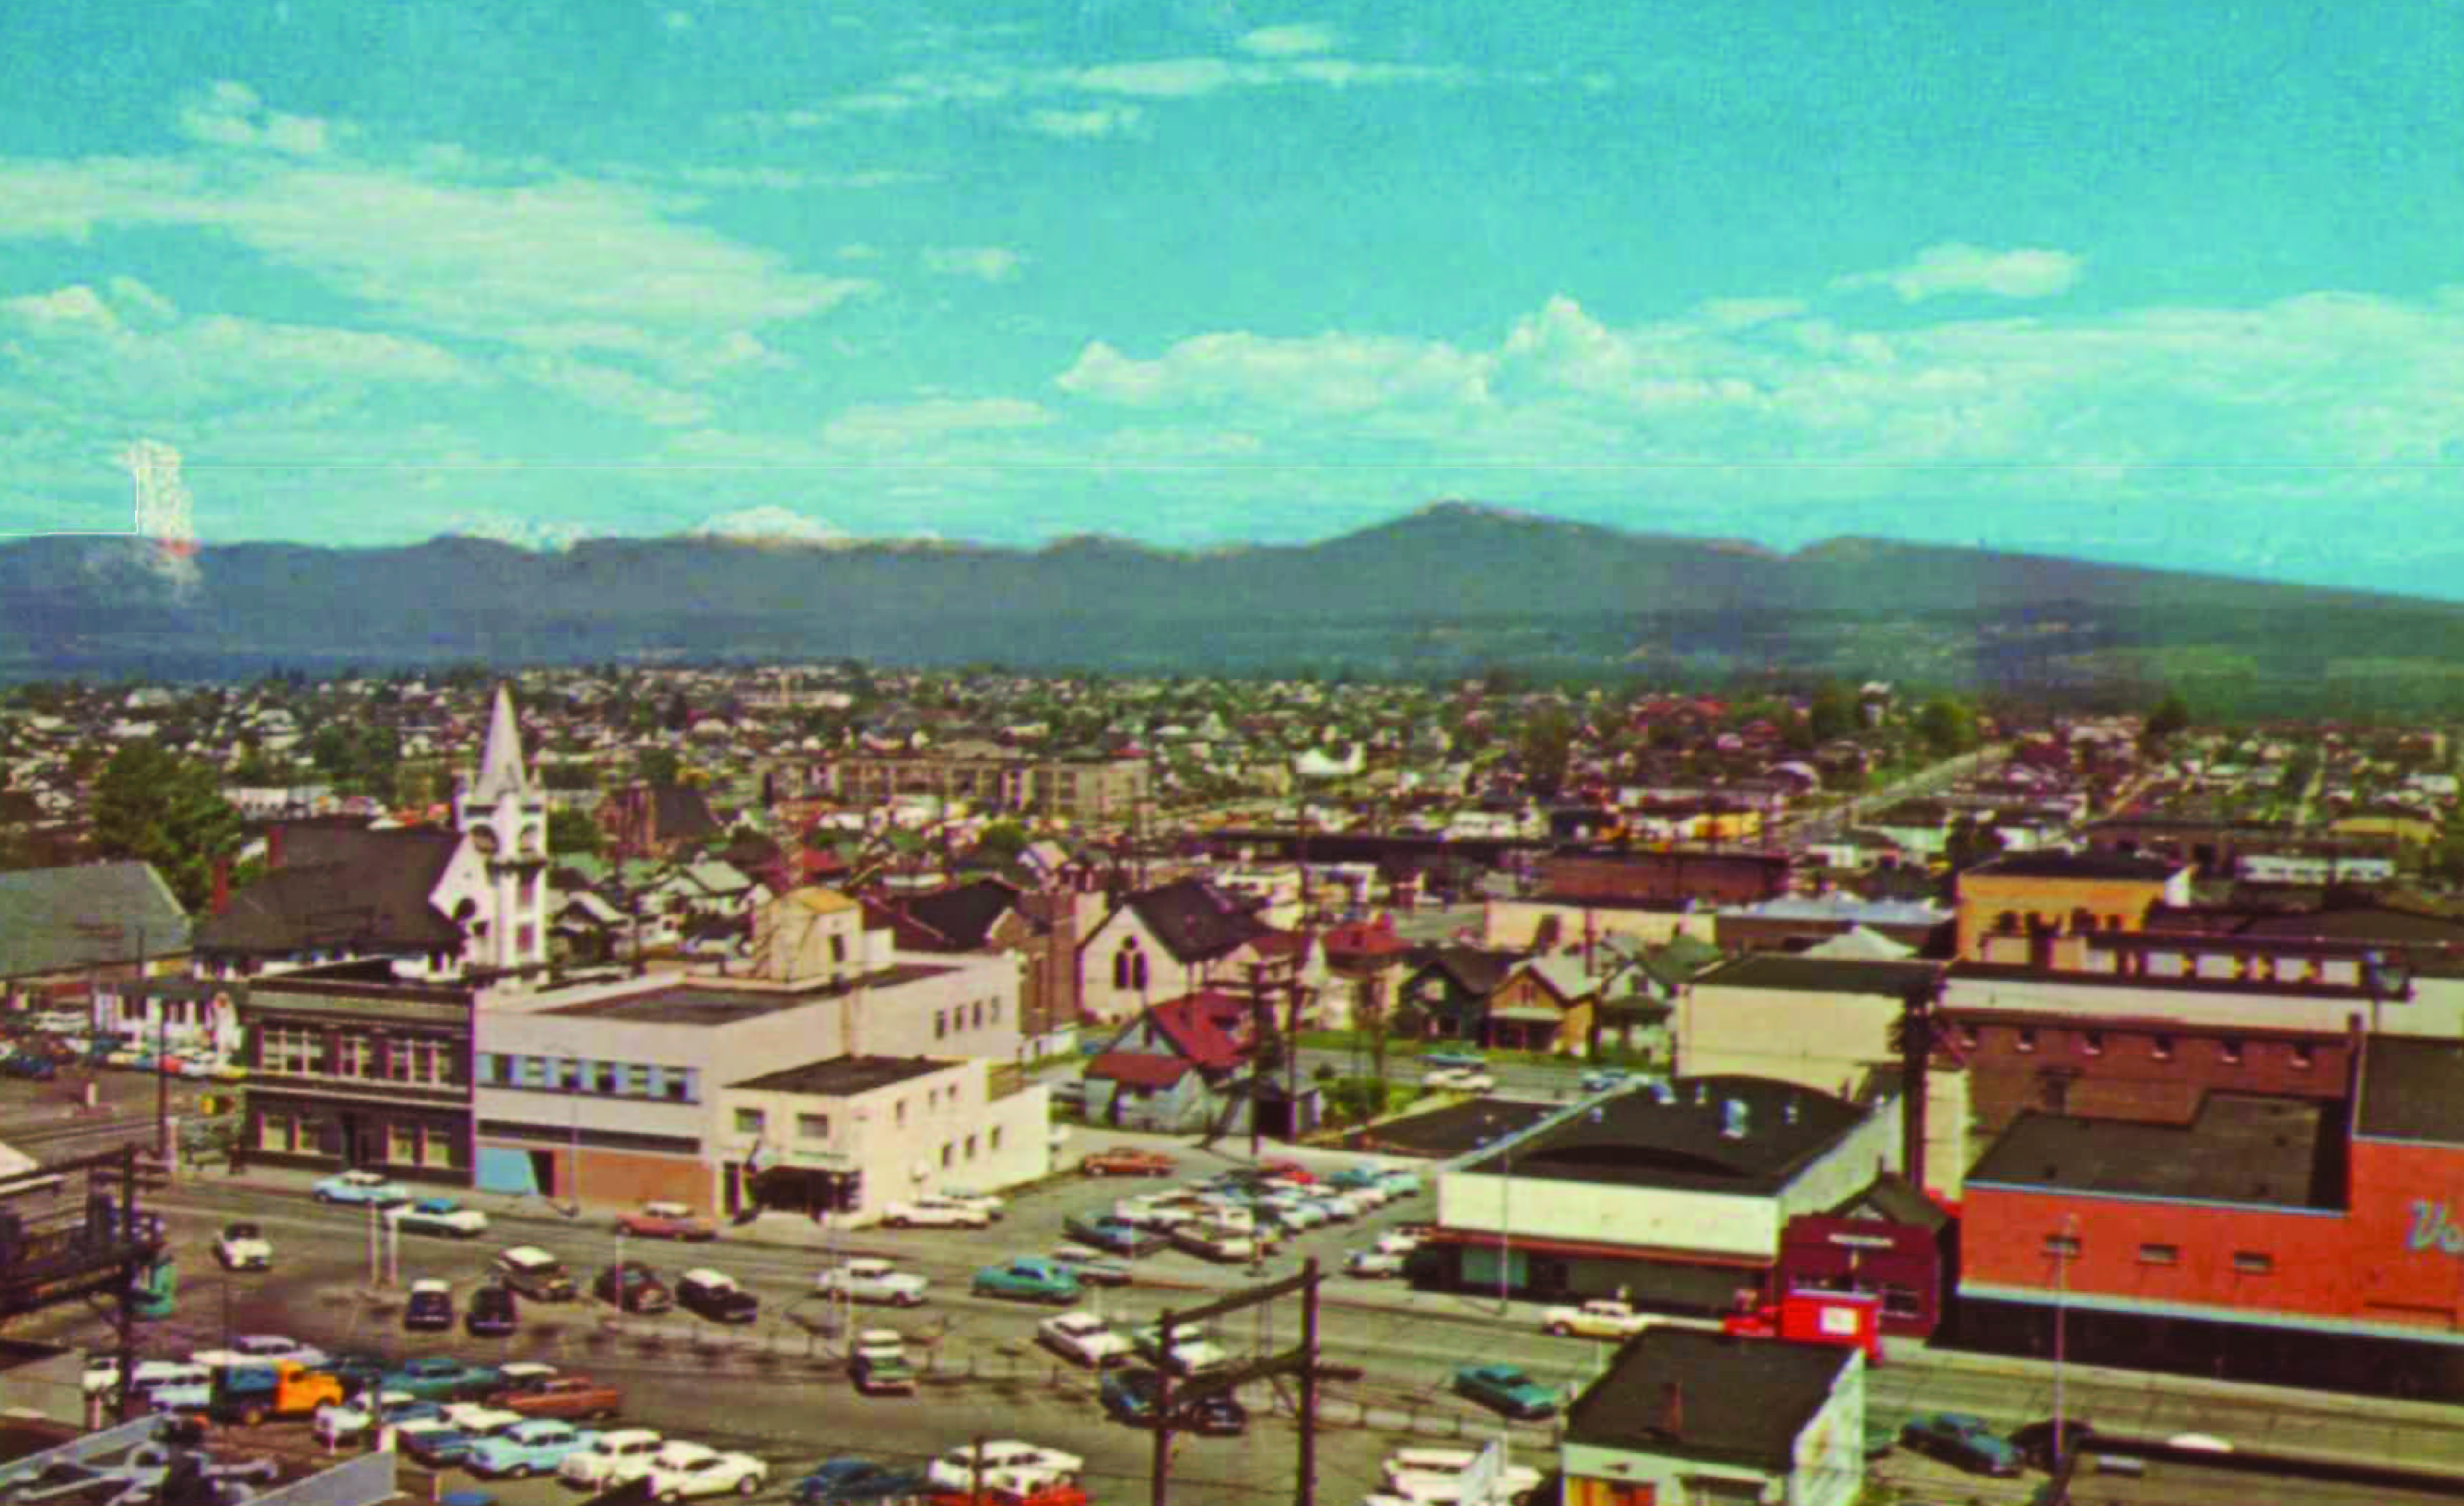
\includegraphics[width=\textwidth, height=\textheight, keepaspectratio]{261-a-mesto_everett}
\caption{Město Everett ve státě Washington v USA. Zde žijí potomci Barbory Prusíkové, provdané Slabé v Šípech}
\label{fig:261-a-mesto_everett}
\end{figure}

             \begin{figure}
\centering
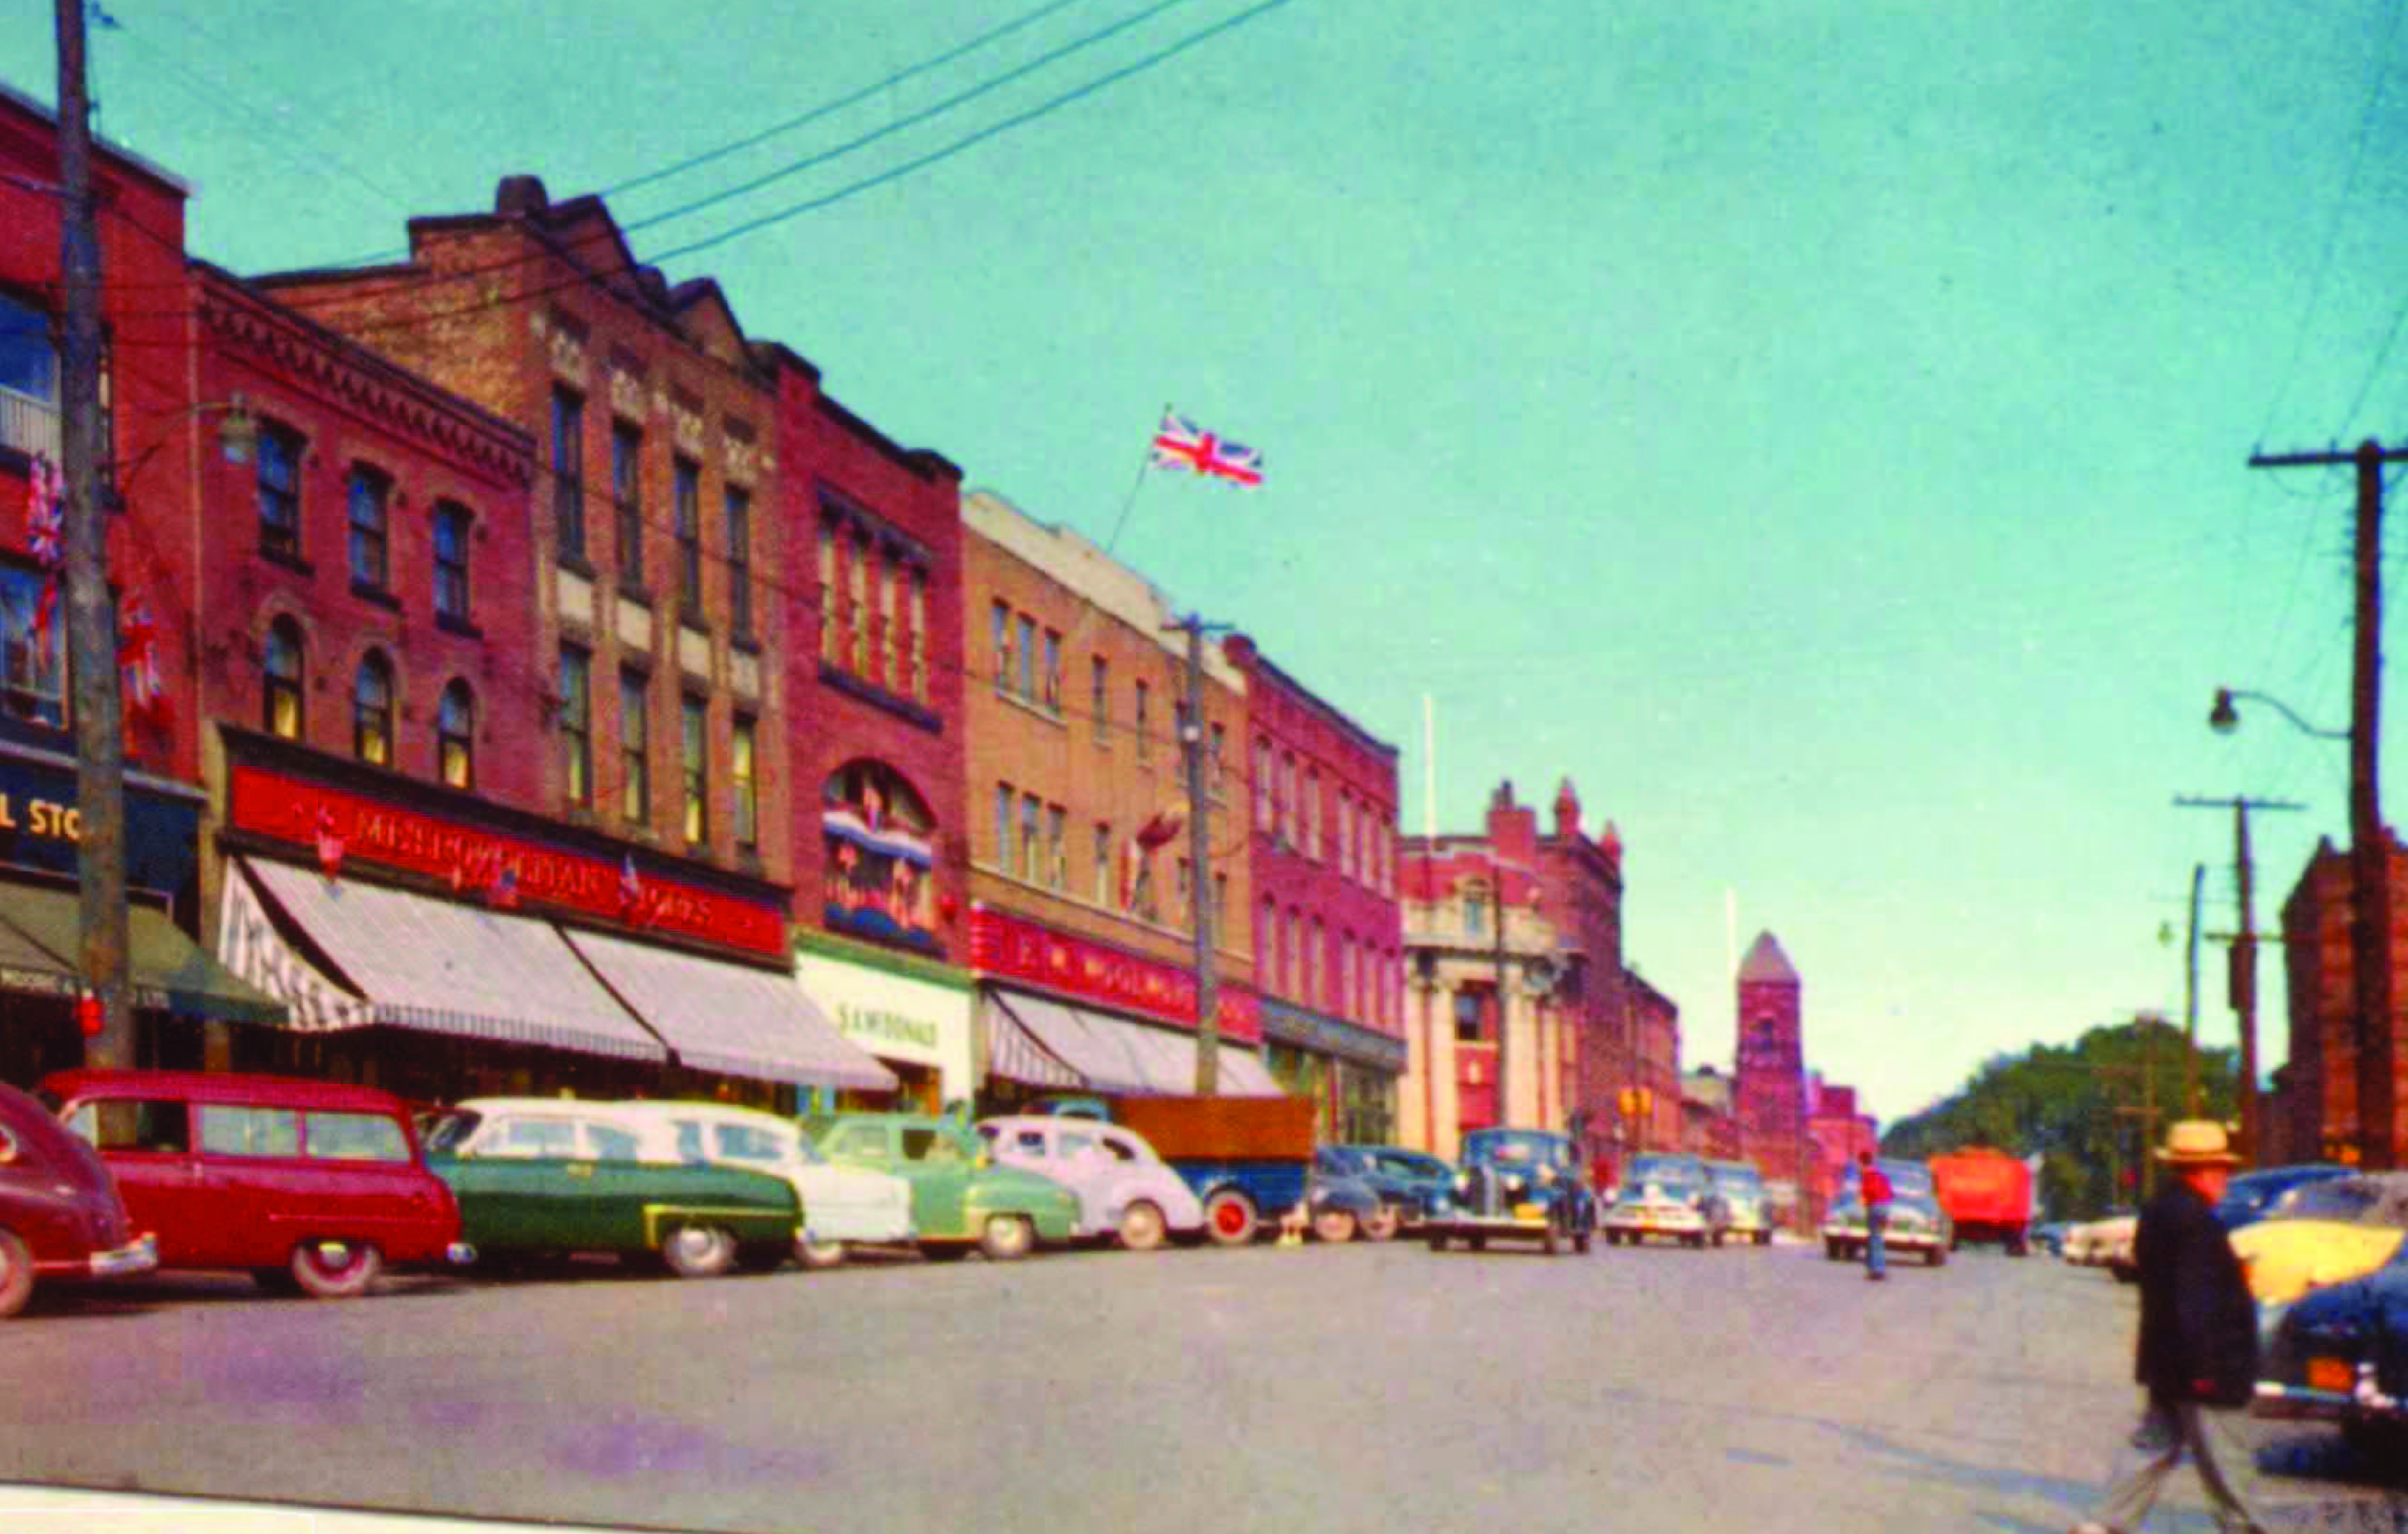
\includegraphics[width=\textwidth, height=\textheight, keepaspectratio]{261-b-charlottetown}
\caption{Pohled na město Charlottetown na ostrově prince Edwarda v Kanadě, kde žije potomek Anny Monséové, rozené Prusíkové ve Stražiště}
\label{fig:261-b-charlottetown}
\end{figure}

% str 224 @ 262 (pokr.)
Nejstarším dítětem byl syn Václav. Narodil se 11. 12. 1864, vyučil se kovářem, žil pak v Dobřanech, ale zemřel v mladém věku 21 let, 1. 11. 1885. Druhým dítětem byla Barbora Prusíková, narozená 28. 9. 1868 v rodišti své matky Snopoušovech. Dne 24. 8. 1889 narodilo se jí nemanželské dítě Barbora. Když se v roce 1893 provdala za Václava Kratochvíla z Brna a tam s ním odjela, bylo její dítě legitimováno a místo Prusíková dostala jméno Kratochvílová. Barbora Kratochví­lová roz. Prusíková zemřela v Brně v mladém věku 28 let 1. 4. 1896.

Její dcera Barbora měla od dětství krušný život. Stala se později ošetřovatelkou v ústavu pro choromyslné v Dobřanech a pak také v Praze-Bohnicích. Již v mládí projevovala literárního ducha, vášnivě milovala knihy a napsala mnoho povídek a básní, zvláště také se zřetelem k životu v "blázincích" a k jejímu těžkému životu v mládí. Provdala se v pozdním věku a žije nyní jako Barbora Czorná v Dobřanech, Jungmannova 719. Její muž je původu ukrajinského a působil u dragounského pluku v Klatovech.

Jako její matka, měla i Barbora Kratochvílová, nemanželské dítě. Je to František Kratochvíl, který se narodil 26. 1. 1915. Je úředníkem ve zdravotnictví. Bydlí v Brně, Klusáčkova 5, kde dříve také dosti dlouho bydlela jeho matka než se provdala a uchýlila do svého rodiště Dobřan. František Kratochvíl má dvě děti. Je to syn Jiří nar. 25. 12. 1952 a dcerka Ivona nar. 25. 9. 1957.

Třetím dítětem bednáře Václava Prusíka byla dcera Matylda. Narodila se 15. 2. 187I v Plzni. Později žila v Dobřanech, tam se seznámila s pekařem Josefem Váňou a s ním se později odstěhovala do jeho rodiště Kamenného Újezdce v Posázaví. Matylda Váňová zemřela na rozdíl od svých dvou sourozenců v pěkném věku 83 let 15. 12. 1954. Měla dvě děti. Dceru a syna. Dcera Anna nar. 19. 7. 1893 (zemřela 6. 4. 1969) provdala se za vojáka Lukáše, který sloužil také v posádce v Dobřanech. Lukášovi měli jediného syna Josefa, narozeného 13. 8. 1920. Jeden čas byl podnikavým obchodníkem, ale nyní je zaměstnán u čsl. aerolinií. Bydlí v Praze 7, Schnirchova 26. První jeho žena mu brzy zemřela a je nyní ženat po druhé. Josef Lukáš má z prvního manželství dvě děti. Syna Josefa nar. 26. 10. 1946 a dceru Jitku nar. 12. 11. 1948. Matylda Váňová rozená Prusíková pak měla ještě syna Jana. Narodil se 5. 2. 1900, byl úředníkem v průmyslu a žil v Sušicích. Po únoru 1948 pomáhal některým postiženým lidem, když se uchylovali za naše hranice a za to byl potrestán dosti dlouhým vězením. To mu zkrátilo život. Po propuštění pracoval v podniku SOLO v Sušici a  tam
% str 225 @ 263
ho zastihla náhlá smrt 11. 9. 1962. Jan Váňa je opravdu obětí doby, neboť sám byl vždy od mládí zaníceným socialistou, ale nebyl nikdy stoupencem násilí. Zanechal po sobě dvě děti. Jeho dcera Božena Váňová nar. 21. 12. 1938 je svobodná a je zaměstnána v textilním obchodě v Sušici, kde bydlí v Leninově ul. 25l. Druhý byl syn Jan Váňa nar. 23. 11. 1934, stal se uči­telem. Zvláštním jeho oborem je matematika a přírodní vědy. Působí a bydlí ve Velharticích na Šumavě č. 123. Má dvě děti, syna Jana nar. 12. 10. 1961 a dcer­ku Šárku nar. 21. 4. 1964.

Posledním dítětem Vojtěcha Prusíka ve Stražišti byl Jan. Narodi1 se 8. 12. 1837 a vyučil se zámečníkem. Odslouži1 si řadu let na vojně a také bojoval v prusko-rakouské válce r. 1866. Dne 24. 2. 1868 se o ženil s dcerou učitele ve Stražišti Janou Legovou. Ta se tam narodila v roce 1840. Útrapy válečné zanechaly však Janovi těžké následky a již za dva roky zemřel bez po­tomků v roce 1870.

\section{Doslov k rodové větvi Stražiště}
Vylíčili jsme vám právě osudy potomků Vojtěcha Prusíka, zednického mistra ve Stražišti, který se tam narodil v roce 1790. Někteří jeho potomci měli pohnutý život a mnohdy také velmi krušný. Dosti značný počet z nich průběhem 150 let ztratili původní českou národnost a žijí dnes v cizině, Německu, Rakousku nebo i za mořem v Kanadě. Je to asi třetina. Hlásí se však všichni ke svému prapůvodu v malé české vesničce.

Vojtěch Prusík, zednický mistr ve Stražišti, který tam zemřel v roce 1867, zanechal až dodnes 160 potomků, z toho dnes již 49 mrtvých. Jen jeden člen rodu z větve Stražiště vynikl nad průměr a jeho jméno se dokonce dnes v celém světě mezi horolezci stalo slovem „prusík“ všeobecně užívaným pojmem. Je to vynálezce horolezeckého uzlu, prof. Dr. Karel Prusík z Vídně, jehož děd Josef tam odjel asi před 120 lety 1848 ze svého rodiště Stražiště. I krásné jeho hudební kompozice jsou zachovány na věčnou paměť na gramofonových deskách a vytištěny. Vždyť hudba byla pro Dr. Karla Prusíka vedle hor tou největší láskou a jako profesor na vídeňské konservatoři vychoval tam několik generací.

Málo je dnes již těch, kdo svým vznikem přísluší do Stražiště a podle této vesničky nazvané větvi a sami tuto obec znají. Bylo by jistě krásné, kdyby aspoň jednou v životě uzřeli místa, která měla pro ně význam i když sami se snad narodili ve většině zcela jinde. Platí to i o vesnici Sedlci u Plas, kde je prapůvod všech nás, kteří krví patříme k prastarému rodu Prusíků.

Nyní si zase na další stránce můžete přečíst jména těch, kdo se narodili se jménem Prusík či Prusíková a jaká jména jiná se průběhem doby vyskytla v této větvi.

% str 226-227 @ 264-265
% TODO seznam

% str 227+1 @ 266
\begin{figure}
\centering
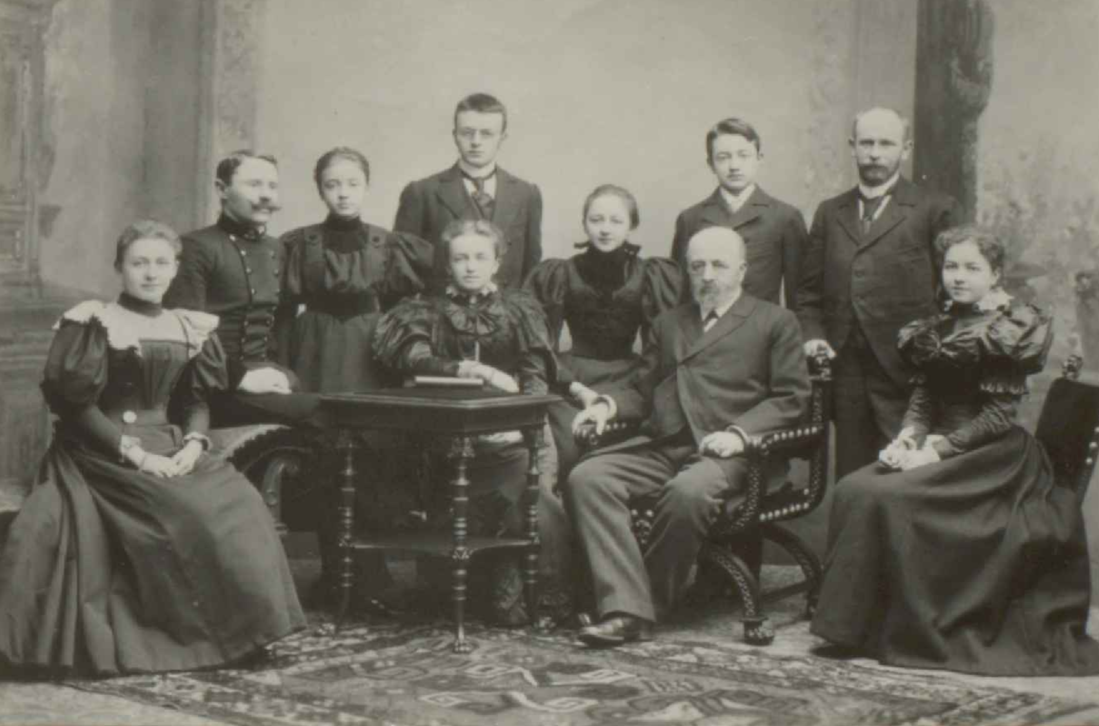
\includegraphics[width=\textwidth, height=\textheight, keepaspectratio]{266-a-rodina_karla_prusika}
\caption{Rodina JUDr. Karla Prusíka, zasloužilého občana města Jihlavy (1840 – 1920)}
\label{fig:266-a-rodina_karla_prusika}
\end{figure}

             \begin{figure}
\centering
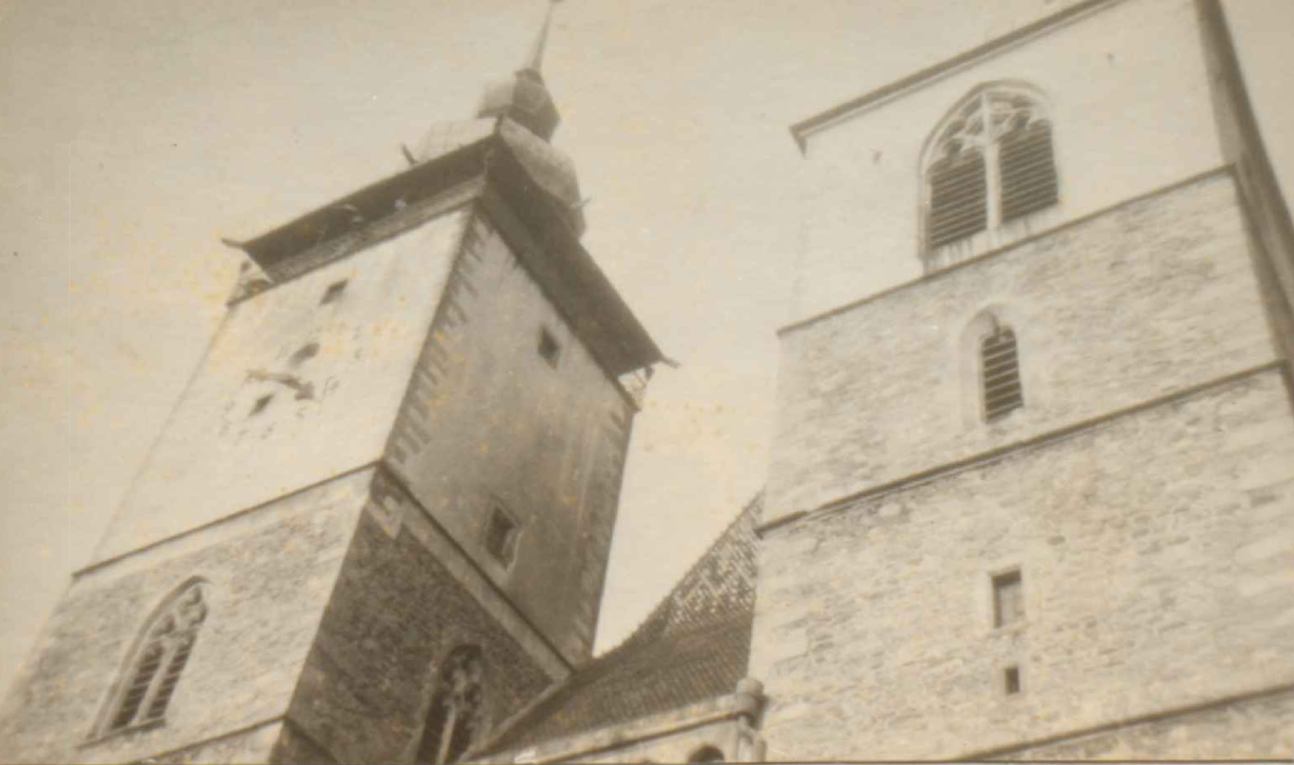
\includegraphics[width=\textwidth, height=\textheight, keepaspectratio]{266-b-kostel_v_jihlave}
\caption{Kostel svatého Jakuba v Jihlavě}
\label{fig:266-b-kostel_v_jihlave}
\end{figure}
\end{document}
